\documentclass{article}
\usepackage[table]{xcolor}
\usepackage{amsmath}
\usepackage{float}
\usepackage{array}
\usepackage{graphicx}
%\usepackage[shortlabels]{enumitem}
\usepackage[spanish, es-tabla]{babel}
\usepackage[utf8]{inputenc}
\usepackage{csquotes}
\usepackage[margin=2cm]{geometry}
\usepackage{wallpaper}
\usepackage[depth=3]{bookmark}
\usepackage[
backend=biber,
style=numeric,
sorting=none
]{biblatex}
\bibliography{references.bib}
% \addbibresource{references.bib} 
\setlength{\parskip}{1em}
\parindent 0px

\newcolumntype{P}[1]{>{\centering\arraybackslash}p{#1}}
\newcolumntype{M}[1]{>{\centering\arraybackslash}m{#1}}
 

\newcommand\signature{
\noindent\begin{minipage}{10cm}
    \noindent\vspace{3pt}\par
    Firma: \rule{7cm}{1pt}
    \noindent\vspace{15pt}\par
\end{minipage}}

\begin{document}

\begin{titlepage}


    \ThisLRCornerWallPaper{1}{imgs/fondo_tt.png} % Fondo de portada 
        \begin{center}
            \huge \textbf{Instituto Politécnico Nacional}\\*[0.3cm]
            \LARGE \textbf{Escuela Superior de Cómputo}\\
            \vspace{1cm}
            %\rule{12cm}{0.5mm}\\*[0.3cm]% Línea {Longitud}{Grosor}
            \hspace{0.9cm}
            \LARGE \textbf{ESCOM}\\
            \vspace{2cm} 
            \Large \emph{Trabajo Terminal}
     
                        %%%%  TITULO Y NÚMERO DE TRABAJO   %%%%
    		\LARGE \textbf{ Aplicación móvil gamificada de aritmética\\}
    		\LARGE \textbf {\emph{ 2021-1-007}} \\
    		\vspace{1cm} %Espacio vertical
    	%\LARGE \textbf{\\ Ingeniería en Sistemas Computacionales\\}
 		\emph{Presentan}\\   	
    	\textbf{Alumnos: Itzcoatl Rodrigo Pineda Vieyra , Izaird Alexander Mothelet Delgado }\\
    	\vspace{3cm}
    	\emph{Directores}\\   	
	Directores: Dra. Lorena Chavarría Báez, Dra. Elena Fabiola  Ruiz Ledesma \\
    \vspace{1cm} %Espacio vertical
        \end{center}

    \centering %Todo centrado
    \vspace{1cm} %Espacio vertical
	
	\begin{flushright}
	\emph{Diciembre 2021}
	\end{flushright}

\end{titlepage}

\tableofcontents
\pagebreak
\section{Introducción}
La intervención educativa requiere de una previa comprensión de la adquisición y desarrollo de la competencia aritmética
que está en la base de todas las posteriores dificultades y trastornos del aprendizaje matemático. Hay dificultades que
pueden surgir a lo largo de este proceso (desde nivel básico), lo que repercute en la resolución de ejercicios y problemas matemáticos avanzados.
Por lo que el desarrollo de la destreza operatoria aritmética es fundamental para que el estudiante, tanto de nivel básico como medio superior, pueda enfrentar con
éxito situaciones más complejas en el campo de la Matemática. Además, se requiere motivar al estudiante al desarrollar
trabajo operatorio aritmético, ya que en ocasiones su desarrollo puede resultar monótono y aburrido. Para ayudar al desarrollo de la destreza operatoria de los estudiantes se propone una aplicación gamificada móvil que promueva la
resolución de ejercicios aritméticos.

\subsection{Motivación}
La Aritmética como la Geometría son de las disciplinas matemáticas más antiguas y necesarias en la historia del género humano \cite{coronado2014estudio}. 
Su utilización funcional es requerida para las personas que participamos de esta sociedad, como medio de comunicación y comprensión de multitud de fenómenos que nos rodean, es por ello que el desarrollo de la destreza operatoria aritmética es una de las habilidades más necesitadas en la alfabetización socio instrumental.
Los niveles de fracaso en el aprendizaje matemático son preocupantes, especialmente en los últimos cursos de escolaridad obligatoria (secundaria). Los resultados de estudios internacionales como el Programa Internacional para la Evaluación de Alumnos de la OCDE (PISA)  \cite{oecd2014what,oecd2016low} muestran que el aprendizaje matemático es el que presenta mayor porcentaje de fracaso \cite{coronado2016academic, mullis2016timss}. El cálculo es un componente esencial en la resolución de problemas aritméticos, y éste es uno de los contenidos más importantes de las matemáticas, junto a la geometría, la medida o la probabilidad. 
Es por ello que un elevado porcentaje de las dificultades de aprendizaje de las matemáticas tiene un origen aritmético, donde el cálculo representa un papel esencial \cite{orrantia2006dificultades}. Las habilidades numéricas y aritméticas son predictores críticos del futuro éxito o fracaso académico matemático \cite{rodriguez2017marcadores}. 

Se ha observado en declive las habilidades operatorias aritméticas de estudiantes universitarios  \cite{tariq2002decline,carpenter2017psychology,huang2013gamification}. 
El estudiante cree que podrá contar con la calculadora de su celular en todo momento, pero cuando esto no se le permite, como en los exámenes de admisión, la falta del entrenamiento del cálculo mental entorpece la solución correcta de los reactivos 
de dichos exámenes. Por otra parte, el no fortalecer la destreza operatoria, afecta diferentes procesos cognitivos al llegar a la edad adulta \cite{martin2003loss}.
El presentar al estudiante los ejercicios de una forma rutinaria muchas veces provoca aburrimiento y desmotivación. 
También es fundamental la motivación y el estado emocional de los estudiantes en su desempeño académico. La motivación y estado emocional de los estudiantes es un factor clave en su desempeño académico \cite{larrazolo2013habilidades,ryan1997should}. Si deseamos que los jóvenes 
mexicanos tengan un mejor desempeño en el área de las Matemáticas, se requiere presentarles 
distintas formas de aprender y practicar sus conocimientos. Para ello una estrategia de 
apoyo es la gamificación, la cual se empleará para incentivar a los estudiantes de educación 
media superior a desarrollar su destreza operatoria.

\subsection{Planteamiento del Problema}
La problemática que se pretende atacar es la necesidad de fortalecer la destreza operatoria aritmética de los estudiantes de medio superior, a través del desarrollo de aplicaciones móviles que incorporen conceptos de gamificación, lo cual es importante para el desarrollo del pensamiento matemático de los estudiantes. 
\subsection{Objetivos}
\subsubsection{Objetivo General}
Desarrollar una aplicación móvil para fortalecer la destreza operatoria en Aritmética, con el uso de la gamificación, con el fin de apoyar al estudiante de medio superior en la adquisición de habilidades y conocimientos elementales.

\subsubsection{Objetivos Específicos}
\begin{itemize}
	\item Diseñar actividades gamificadas, empleando números naturales con las 4 operaciones básicas.
	\item Desarrollar un módulo evaluador de expresiones, para la creación de preguntas que se presentaran a los usuarios.
	\item Desarrollar un módulo de logros y mecánicas.
	\item Validar la aplicación móvil. 
\end{itemize}
\subsection{Estado del Arte}
El trabajo realizado en torno a la gamificación en los últimos años es considerablemente extenso, siendo aplicado en diferentes ambientes, demográficas y propósitos. El presente documento se enfoca en el trabajo relacionado a su aplicación en el ámbito matemático.

En Brasil se creó una plataforma  interactiva en linea enfocada en ayudar a estudiantes de nivel medio en sus lecciones de matemáticas y como entrenamiento para la Olimpiada Brasileña de Escuelas Públicas (Olimpiada Brasileira de Matematica das Escolas Pablicas - OBMEP). El sistema permite a los alumnos resolver problemas generados aleatoriamente y divididos en tres temas principales, que son: Aritmética, Geometría y Combinatoria. El sistema pretende que el alumno resuelva un número determinado de problemas para entender los algoritmos y la lógica que hay detrás. También está vinculado con conceptos de gamificación para involucrar a los estudiantes en las actividades propuestas \cite{toda2014project}.

En un estudio canadiense se propone una familia de rompecabezas que gamifican la práctica de la aritmética. Los rompecabezas se diseñan con un algoritmo evolutivo que constituye una instancia de generación automática de contenidos. Se definieron dos clases de rompecabezas: aquellos en los que la solución óptima utiliza todas las piezas y aquellos en los que la solución óptima no utiliza al menos una pieza\cite{foxcroft2020polyomino}.

En otro estudio \cite{jaguvst2018examining} se experimentó con tres tipos diferentes de actividades de aprendizaje gamificado (competitivo, colaborativo y adaptativo), en alumnos de segundo grado y de tercero que utilizaban tabletas y lecciones de aprendizaje digital para aprender matemáticas.Los niveles de rendimiento fueron significativamente más altos en una condición de gamificación que combinaba competición, narrativa y adaptabilidad con elementos de juego de rendimiento individual. Concluyen con el hecho de que la gamificación funcione o no no es el resultado de los elementos individuales del juego, sino la consecuencia de su combinación equilibrada.
 
Un estudio argentino \cite{zimmerman2016arithmetic} desarrolló una aplicación Android llamada Moravec con 150 niveles con 20 problemas cada uno, donde se requieren 15 respuestas correctas en determinado tiempo para avanzar al siguiente nivel. Concluyen que se puede motivar a los participantes a realizar un entrenamiento aritmético sustancial simplemente presentándolo en un formato gamificado .

En la tabla 1 se presentan aplicaciones similares disponibles en la Appstore.

\begin{table}[H]
\caption{Comparación con softwares disponibles.}
\centering
\begin{tabular}{|c|M{6cm}|M{5cm}|}
\hline
Software & Características & Precio en el mercado \\ \hline

Fraction Challange & 
\begin{itemize}
	\item PVP(Player versus Player) Jugador versus Jugador local
	\item rondas con tiempos
\end{itemize} & 
Gratuito con micro transacciones \\ \hline


1+2=3 & 
\begin{itemize}
	\item Sumas y restas de enteros
	\item Tablas de liderato 
\end{itemize}& 
Gratuito \\ \hline


Fracciones calculadora & 
\begin{itemize}
	\item Calculadora de fracciones
\end{itemize}& 
Gratuito \\ \hline


Math Games & 
\begin{itemize}
	\item Logros
	\item Tablas de liderato
	\item Estadísticas
	\item Tutoriales de como realizar operaciones básicas
\end{itemize} & 
Gratuito con contenido bloqueado (se puede desbloquear haciendo un pago único) \\ \hline

Arithmetic Practice & 
\begin{itemize}
	\item Logros
	\item Tablas de liderato
\end{itemize} & 
Gratuito con contenido bloqueado (se puede desbloquear haciendo un pago único) \\ \hline


Mental Arithmetic  & 
\begin{itemize}
	\item PVP local
	\item Logros
	\item Tablas de liderato
	\item Estadísticas
	\item Contenido desbloqueable
\end{itemize} & 
Gratuito \\ \hline

\end{tabular}
\label{tab:software}
\end{table}
\subsection{Propuesta de Solución}
Con este proyecto se pretende ayudar al desarrollo de la destreza operatoria en la resolución de ejercicios aritméticos con números naturales haciendo uso de ciertos componentes de la gamificación (Logros) y mecánicas (Competición). Como futuros ingenieros en sistemas computacionales tenemos la responsabilidad de usar las habilidades para un beneficio social, por lo que deseamos unir esfuerzos para apoyar al estudiante a mejorar su destreza operatoria.
Los ejercicios podrán presentarse empleando preguntas de opción múltiple según la preferencia del usuario,
con la puntuación cambiando correspondientemente. Se contará con un sistema de puntuación basado en el tiempo de
respuesta para medir el desempeño. Esto con el propósito de fomentar la competitividad, permitiendo al estudiante llevar
un registro del progreso de su puntuación.
%\section{Marco Teórico}
%\section{Aritmética}
\section{Importancia de la Aritmética}
El aprendizaje de las matemáticas supone, junto a la lectura y la escritura, uno de los aprendizajes fundamentales de la educación, de ahí que entender las dificultades en el aprendizaje de las matemáticas se haya convertido en una preocupación manifiesta por profesionales dedicados al mundo de la educación, especialmente si se considera el alto porcentaje de fracaso que presentan en estos contenidos los alumnos que terminan la escolaridad obligatoria \cite{pisa2010results}. 

Antes, es necesario acotar lo que se entiende por dificultades en el aprendizaje de las matemáticas, puesto que los contenidos de matemáticas pueden ser muy diversos. Así, las dificultades pueden aparecer en contenidos como la Geometría, la Probabilidad, la medida, el Álgebra o la Aritmética. Pero se está de acuerdo en que es en la Aritmética donde los alumnos encuentran sus primeras dificultades, puesto que estos son los contenidos a los que se enfrentan en primer lugar, además de que son la base sobre la que se asientan los demás contenidos. 

Por lo señalado en los dos párrafos previos, esta sección inicia comentando cómo se adquieren y que desarrollo siguen los contenidos aritméticos básicos, distinguiendo entre aquellos que surgen desde la experiencia informal, es decir, que no implican una enseñanza explícita, y los que se adquieren a través de la enseñanza formal. En los primeros se abordan algunos aspectos del desarrollo del número, considerando dos elementos clave: el conteo y los esquemas de razonamiento protocuantitativos. Posteriormente se muestran situaciones problemáticas a las que los alumnos se enfrentan de manera formal, así como las estrategias de conteo que utilizan para su resolución.
\subsection{El desarrollo de la Aritmética desde el aspecto cognitivo}
\subsubsection{Aritmética informal: las primeras nociones aritméticas}
Hablar del desarrollo de la aritmética en particular o del desarrollo del pensamiento matemático en general implica mencionar, aunque sea brevemente, los planteamientos piagetianos sobre esta cuestión.

Para Piaget \cite{piaget2015psicologia} el conocimiento matemático se desarrolla como consecuencia de la evolución de estructuras más generales, de tal manera que la construcción del número es correlativa al desarrollo del pensamiento lógico y se relaciona con la aparición del estadio operacional donde aparecen los requisitos lógicos del número, el cual ocurre aproximadamente entre los 6 y los 12 años de edad. En una edad más temprana (de los 3 a los 6 años), el niño no piensa de forma operatoria, dado que cuando han acabado de ejecutar una acción no son capaces de recordar el aspecto que tenía antes. En términos piagetianos no han conseguido la reversibilidad. Entonces entre los 3 y 6 años los niños se ubican en el estadio denominado preoperacional o preoperatorio, en el que su pensamiento está dominado por datos perceptuales, como se demuestra en sus famosos trabajos sobre la conservación y la clasificación. 

En un experimento típico de la conservación se presenta al niño por ejemplo dos filas de fichas, una con fichas azules y otra con fichas rojas, en correspondencia biunívoca, y a continuación se separan las fichas de una de las filas ante los ojos del niño. Los niños preoperatorios ya no consideran que las dos filas tengan el mismo número de fichas. Esto ocurre porque cuando se separan las fichas el niño no es capaz de imaginárselas en su posición original, guiándose a la hora de hacer juicios por variables perceptivas.

Por otro lado, en los experimentos sobre clasificación se enseña por ejemplo un conjunto con dos bolas de madera rojas y siete azules. Los niños son capaces de decir que son todas de madera y que hay más bolas azules que rojas. Sin embargo, cuando se les presenta la pregunta "¿qué hay más: bolas azules o bolas de madera?", los niños preoperatorios dicen que hay más bolas azules, dado que el dominio perceptivo de la cantidad de bolas azules interfiere con la consideración de que todas son de madera; parece incapaz de comparar un subconjunto con su propio superconjunto.

Es precisamente en el estadio de las operaciones concretas donde desaparece esta dependencia de las variables perceptivas o esta incapacidad para pensar de forma reversible. En este estadio aparece la adquisición del pensamiento lógico, la comprensión de las clases, las relaciones y las correspondencias biunívocas. En definitiva, un verdadero concepto del número y una manera significativa de contar. Desde este punto de vista, el desarrollo del número es para Piaget una cuestión de "todo o nada", puesto que, hasta que no cuente con los conceptos lógicos, el niño va a ser incapaz de comprender el número y la aritmética.

Sin embargo, están apareciendo cada vez más autores que no están de acuerdo con este enfoque del desarrollo del número, y que piensan que los niños pueden aprender mucho acerca de contar, del número y de la aritmética antes de poder conservar.

A raíz del influyente trabajo de Gelman y Gallistel \cite{german1978child}, sobre el desarrollo temprano del conteo, se empezó a demostrar que, contrario a lo que pensaba Piaget, el conteo juega un papel importante en el desarrollo del número y de las primeras nociones aritméticas, y que los niños preescolares muestran una sorprendente competencia cognitiva en este campo.

Sin embargo, el primer conocimiento numérico es posible que se origine, como así han demostrado algunas investigaciones \cite{carpenter2020development,kintsch1985understanding}, antes de que los niños dispongan del conteo verbal transmitido culturalmente o de cualquier otra influencia social. O lo que es lo mismo, que puede haber un origen innato del número, similar a muchas habilidades perceptivas.

Sin embargo, y aunque estas primeras nociones del número son importantes, es a partir de los tres años de edad cuando los niños comienzan a desarrollar el primer conocimiento cuantitativo \cite{orrantia2003rol}. En este desarrollo hay dos elementos que juegan un papel importante, el conteo verbal y los esquemas protocuantitativos \cite{resnick2020protoquantities}. Concretamente, desde la integración de estos dos aspectos los alumnos son capaces de enfrentarse a la resolución informal de las primeras situaciones problemáticas.
\subsubsection{El conteo verbal}
A pesar de que los contextos sociales que rodean al niño pueden variar de unas culturas a otras, lo cierto es que todas ellas ofrecen un sistema de palabras numéricas, a veces altamente elaborado como nuestro sistema de base diez, además de las oportunidades para manipular y contar pequeñas cantidades discretas de objetos. No cabe duda de que este primer conocimiento numérico aportado por la cultura juega un papel importante en el desarrollo del pensamiento matemático de los niños.

Sin embargo, y a pesar de que el conteo parezca una actividad sencilla a los ojos de un adulto, lo cierto es que en realidad necesita de la integración de una serie de técnicas que se desarrollan con el tiempo. Por ejemplo, se requiere determinar si un conjunto de nueve puntos es mayor o menor que uno de ocho. En primer lugar, se necesita generar los nombres de los números en el orden adecuado. Además, se deben aplicar las etiquetas de la serie numérica una por una a cada objeto de un conjunto; para ello, es necesario coordinar la verbalización de la serie numérica con el señalamiento de cada elemento del conjunto para crear una correspondencia entre las etiquetas y los objetos. En tercer lugar hay que representar los elementos que contiene cada conjunto, para lo que se necesita la \emph{regla del valor cardinal}, por la que se establece que la última etiqueta expresada en la serie numérica representa el número total de elementos del conjunto. Por último, es preciso comprender que la posición de un número en la secuencia define la magnitud, de tal forma que se pueda establecer que el nueve viene después del ocho y por lo tanto es más grande.

Por lo tanto, desde el punto de vista cognitivo, el conteo no es una tarea sencilla, constituyendo un enorme reto para los niños de corta edad. Y su adquisición es un largo proceso que posiblemente no culmine hasta los siete u ocho años de edad.

Para una comprensión plena del número para tareas de cuantificación se requiere el desarrollo del conocimiento de los principios sobre el conocimiento conceptual del conteo, los cuales son: los principios de correspondencia uno-a-uno, de orden estable, de cardinalidad, de abstracción y de irrelevancia, y fueron desarrollados en el trabajo pionero de Gelman y Gallistel \cite{german1978child}.

\textbf{El principio de correspondencia uno-a-uno}  implica etiquetar cada elemento de un conjunto una vez y solo una. Conlleva, por tanto, la coordinación de dos procesos: partición y etiquetación, de tal manera que los niños mediante la partición van controlando los elementos contados y los que quedan por contar, bien separándolos o bien señalándolos, a la vez que disponen de una serie de etiquetas de modo que cada una de ellas corresponda con un objeto del conjunto contado. 

\textbf{El principio de orden estable}estipula que para contar es imprescindible el establecimiento de una secuencia coherente, aunque, como indican Gelman y Gallistel \cite{german1978child}, este principio se puede aplicar sin necesidad de tener que utilizar la secuencia numérica convencional, pudiéndose utilizar una secuencia propia no convencional, pero siempre de manera coherente.

\textbf{El principio de cardinalidad} establece que la última etiqueta de la secuencia numérica representa el cardinal del conjunto, esto es, la cantidad de elementos que contiene el conjunto. Gelman y Gallistel \cite{german1978child} consideran que los niños comprenden este principio si repiten o ponen un énfasis especial en el último elemento de la secuencia de conteo.

\textbf{El principio de abstracción} determina que los principios anteriores se puedan aplicar a cualquier tipo de conjunto, tanto con elementos homogéneos como heterogéneos (objetos de distinto color o distinta entidad física).

\textbf{Por último, el principio de irrelevancia }indica que el orden por el que se comience a enumerar los elementos de un conjunto es irrelevante para su designación cardinal. Así, se puede contar de izquierda a derecha, de derecha a izquierda o del centro hasta los extremos sin que ello afecte al resultado del conteo.

Los principios de correspondencia, estabilidad del orden y cardinalidad establecerían las reglas procedimentales sobre cómo contar un conjunto de objetos. A partir de sus experiencias con el conteo el niño va adquiriendo la secuencia numérica convencional, y esto le va a permitir establecer cuántos elementos tiene un conjunto, lo que se conoce con el nombre de enumeración.

La abstracción y la irrelevancia del orden sirven para generalizar y flexibilizar el rango de aplicación de los principios anteriores, lo que otros han llamado características no esenciales del conteo. Por ejemplo, es común que un niño considere como característica esencial el contar de izquierda a derecha, de tal forma que cuando se comienza a contar por el centro lo consideran un error. Esto significa que no ha adquirido el principio de irrelevancia.

\subsubsection{Los esquemas protocuantitativos}
Paralelamente a la habilidad de contar, los niños van desarrollando cierta experiencia con distintas formas de relaciones numéricas que son importantes para el desarrollo posterior del número y la aritmética. Estas relaciones han sido definidas por Resnick \cite{resnick2020protoquantities,resnick1989developing} como \emph{esquemas protocuantitativos}. De esta forma esta autora hace una distinción entre dos tipos de conocimientos, lo que ella llama conocimiento representacional o conteo, y conocimiento relacional, caracterizado por los esquemas protocuantitativos. Desde el punto de vista de Resnick \cite{resnick2020protoquantities,resnick1989developing} estos dos tipos de conocimientos tienen orígenes separados en el desarrollo temprano del número, y solamente a través de su integración se ejecuta el conocimiento cuantitativo.

Al igual que ocurre con el desarrollo del lenguaje, en el desarrollo del conocimiento matemático el niño va disponiendo de una variedad de términos que expresan juicios de cantidad sin precisión numérica, como mayor, menor, más o menos, lo que les permite asignar etiquetas lingüísticas a la comparación de tamaños. Estos juicios, que operan sin ningún proceso de medida, se basan en lo que Resnick  \cite{resnick2020protoquantities,resnick1989developing} llama esquema protocuantitativo de comparación. Esta autora identifica dos esquemas protocuantitativos más: uno que interpreta cambios en las cantidades como un incremento o decremento y otro que establece relaciones parte-todo.

El esquema protocuantitativo incremento-decremento permite a los niños de tres años razonar sobre cambios en las cantidades cuando se les añade o se les quita algún elemento. Por ejemplo, un niño sabe que si tiene cierta cantidad de cualquier cosa, por ejemplo dos juguetes, y consigue otro juguete tiene más que antes. De la misma manera que si le quitan tiene menos, o si no le añaden o quitan tiene la misma cantidad aún en el caso de que se modifique la distribución espacial de los objetos.

Por otro lado, y desde el esquema protocuantitativo parte-todo, los preescolares son capaces de conocer que cualquier "pieza", por ejemplo un pastel, puede ser dividida en partes más pequeñas y que volviéndolas a juntar dan lugar a la pieza original. De la misma manera, se pueden juntar dos cantidades que dan lugar a una cantidad mayor, de tal forma que, por lo menos de manera implícita, los niños empiezan a conocer la propiedad aditiva de las cantidades; pueden saber que el todo es mayor que las partes.

De manera que cuando se integra el conocimiento relacional con el conocimiento representacional (el conteo) se desarrollan las habilidades implicadas en la resolución de distintas situaciones problemáticas. Por plantearlo de otra manera, el conteo supondría la cuantificación de los esquemas protocuantitativos a través de la resolución de situaciones problemáticas. 

\subsubsection{Estrategias de conteo}
Las primeras situaciones de suma y resta a que se enfrentan los niños en la etapa infantil y primer curso de la etapa primaria pueden ser resueltas por el modelado directo, esto es, a partir de modelar directamente la situación o acción con objetos físicos, como cubos, los dedos o simplemente dibujando sobre el papel. Los objetos son utilizados para representar la situación y los números de las cantidades dadas en la misma, así como para ayudar al niño a llevar a cabo el procedimiento para llegar a la solución.

De esta forma, con conocimientos mínimos sobre el número y el conteo, y con el conocimiento relacional de los esquemas protocuantitativos, los niños son capaces de resolver numerosas situaciones problemáticas. Para ello hacen uso de diferentes estrategias que modelan la situación y les permiten llegar a la solución.

Con el tiempo, y especialmente con el desarrollo conceptual del conteo, los niños van descubriendo espontáneamente o bien desde la inducción, estrategias de conteo más sofisticadas, abstractas y eficientes que les permiten llegar más rápidamente a la resolución de la situación problemática. Además, hay una transición desde la utilización de materiales concretos o dedos al conteo verbal o mental, por lo que los niños comienzan también a desarrollar procedimientos que les permitan llevar la cuenta de los elementos contados. 

Una estrategia similar, aunque aparentemente algo más avanzada, es la denominada \emph{contar a partir del mayor}, en la que el inicio del conteo se lleva a cabo a partir del conjunto que incluye el sumando mayor, y no el primero. 

Es importante tener en cuenta que para utilizar una estrategia en la que el conteo comienza a partir de uno de los conjuntos es necesario contar con una serie de requisitos, los cuales están relacionados con el desarrollo del conocimiento conceptual del conteo. Así, el primer requisito y más evidente es poder comenzar el conteo a partir de cualquier punto arbitrario de la serie numérica. Otros requisitos tienen que ver con el significado de las relaciones entre conteo y cardinalidad.

Por lo que se refiere a las situaciones de resta, también aparecen dos estrategias más abstractas y evolucionadas: el retroconteo y la cuenta progresiva \cite{fuson1996levels}. El retroconteo es una estrategia inversa a contar a partir de uno de los conjuntos, dado que supone contar en orden contrario al conteo habitual o contar hacia atrás. Por ejemplo, cuando a un conjunto de nueve elementos le quitamos cuatro, caso de un problema de cambio en el que se pide el conjunto final o resultado, los niños pueden hacer lo siguiente: "nueve; ocho (que es uno menos), siete (que es dos menos), seis (que es tres menos), cinco (que es cuatro menos) -cinco", mientras van señalando los objetos del conjunto que se va quitando, o se van sacando dedos hasta formar este conjunto. A diferencia de las estrategias revisadas anteriormente para la suma, el retroconteo no es solamente un procedimiento abreviado de la estrategia menos madura de separación; además se necesita un dominio de la serie numérica en ambas direcciones, puesto que en la estrategia de separación todos los conteos son hacia adelante.

La cuenta progresiva, sin embargo, es una estrategia utilizada en la resta que utiliza el conteo hacia adelante, aunque conceptualmente se aleja de la idea de resta como quitar o separar. En este caso se parte del conjunto más pequeño y se cuenta hacia adelante hasta llegar al conjunto mayor. Por ejemplo si tenemos 8-3, los niños dirían: “tres; cuatro, cinco, seis, siete, ocho;-ocho”, con algún procedimiento para llevar la cuenta de los elementos contados, por ejemplo usando los dedos de la mano.

El siguiente paso en el desarrollo de las estrategias consiste en recuperar directamente desde la memoria el resultado de la operación, lo que se llama \emph{recuperación de hechos} (p.e. siete más nueve es dieciséis) o la utilización de \emph{hechos derivados} (p.e. siete más nueve es igual que diez más seis). En este nivel aparece la composición aditiva, que permite descomponer cualquier número en otros dos (p.e. el siete incluye el cuatro y el tres; o el dos y el cinco; o el seis y el uno; etc). Esto permite operar con el concepto parte/todo, en el que cualquier triada numérica se puede integrar dentro de un esquema sumando-sumando-suma. La suma es entonces vista como cualquier situación en la que dos sumandos son conocidos, y la resta como cualquier situación en que se conoce la suma y uno de los sumandos. Y esto permite la aparición de la reversibilidad entre la suma y la resta, lo que supone una enorme flexibilidad en la resolución de cualquier situación problemática.

En resumen, en lo que se ha llamado aritmética informal, los niños desarrollan una serie de conocimientos conceptuales y procedimientos que les permiten enfrentarse a numerosas tareas aritméticas, especialmente las planteadas como resolución de situaciones problemáticas, donde el conteo juega un papel fundamental. A partir de estos conocimientos, o mejor dicho, conectando con ellos, comienza el aprendizaje de la aritmética más formal.

\subsection{Aritmética formal} 
En el proceso de enseñanza-aprendizaje de la aritmética más formal, se considera el  proceso de resolución de problemas propiamente dicho y el cálculo de operaciones. Debido a que el presente trabajo terminal aborda lo referente a las operaciones básicas, enseguida se comenta al respecto.
\subsubsection{Operaciones básicas}
Llega un momento en que los alumnos comienzan a dominar las combinaciones numéricas básicas, es decir, a recuperar directamente el resultado desde la memoria, lo que se llama recuperación de hechos, lo cual se ve favorecido con la presión por parte de los profesores para que sus alumnos pasen rápidamente del conteo a la recuperación inmediata de hechos aritméticos.

Pero la memorización de las combinaciones numéricas no es lo mejor, es preferible que el estudiante use estrategias de conteo para descubrir relaciones matemáticas que pueden actuar como reglas para generar las combinaciones numéricas. Incluso, algunos autores \cite{fuson1996levels}, consideran que muchas combinaciones numéricas se aprenden y se representan en la memoria no como hechos separados sino como reglas que relacionan distintas combinaciones. Por ejemplo, la regla del cero y la regla del más uno o número siguiente para la suma implican no tener que aprenderse todas las combinaciones que incluyan más cero o más uno, puesto que estas combinaciones se pueden generar por reglas como \emph{todos los números más cero son el mismo número} o \emph{todos los números más uno son el número siguiente}. Algo similar ocurre en la resta, con reglas como N - N siempre es 0, o N - 0 siempre es N, o restas con términos seguidos siempre es 1 (p.e. 7 - 6, 9 - 8, 35 - 34...).

Independientemente de que la representación de hechos en la memoria sea mediante reglas o sean hechos aislados, lo que sí parece indudable es que estas reglas pueden jugar un papel importante en el aprendizaje de las combinaciones numéricas básicas. Y también parece un hecho constatado que antes de la recuperación automática de hechos desde la memoria, las respuestas a combinaciones numéricas desconocidas se pueden generar mediante estrategias de hechos derivados.

Por estrategias de hechos derivados (también llamadas estrategias de pensamiento, estrategias heurísticas o soluciones indirectas) se entienden aquellos procedimientos en los que los números en una operación dada se redistribuyen de tal forma que se convierten en números cuyas sumas o diferencias son conocidas. Por ejemplo, la operación 6 + 7 se puede simplificar descomponiendo los números para generar hechos conocidos, como los dobles más uno ([6 + 6] + 1; si seis más seis son doce, y siete es uno más que seis, entonces seis más siete es uno más que doce, esto es, trece). O también utilizar la redistribución basada en el diez, muy utilizada en las combinaciones en las que uno de los sumandos sea nueve, como 9 + N o N + 9; en este caso, la combinación es descompuesta para hacer que uno de los sumandos sea diez; así, 9 + 6 se puede descomponer en 9 + [ 5 + 1] para dar 9 + 1 = 10 + 5. En el caso de la resta, cualquier combinación puede resolverse, entre otros procedimientos, recordando su combinación aditiva complementaria; por ejemplo, 8 - 5 se puede resolver pensando que se necesita añadir a cinco para hacer ocho (5 + 3 = 8); por lo tanto, las combinaciones numéricas básicas aditivas preceden en el tiempo a las de la resta.

Estas estrategias de hechos derivados también pueden utilizarse en el dominio de las combinaciones numéricas de multiplicación y división. Por ejemplo, la regla del cero en 7 X 0 se entiende como siete grupos de nada es nada; y la regla de multiplicar por uno como un grupo de siete elementos es siete.

No cabe duda de que estas reglas y procedimientos pueden constituir un andamiaje para la recuperación inmediata desde la memoria de hechos numérico. Ahora bien, ¿qué tan importante es la práctica en este contexto?, algunos autores \cite{orrantia2002dificultades} consideran que  la práctica  puede favorecer la utilización de manera cada vez más automática de estas reglas, principios y estrategias de pensamiento. Es por ello que en este trabajo terminal se trabaja esa práctica mediante la utilización de algunos aspectos de la gamificación.

\subsubsection{Dificultades en la Aritmética} 
Una vez analizados los contenidos de la aritmética desde el punto de vista del proceso de desarrollo que siguen los niños, en este apartado se analizan algunas de las dificultades que pueden surgir en este proceso. Antes, sin embargo, es conveniente  plantear una fuente de dificultades que no suele mencionarse, posiblemente por lo inespecífica que es. Se refiere a la desconexión que muchas veces existe en la enseñanza de la aritmética entre el conocimiento informal que los niños desarrollan espontáneamente y los conocimientos más formales que aprenden en las aulas.

Como se ha revisado a lo largo de este segundo capítulo del Trabajo Terminal, los niños desarrollan, antes de la enseñanza formal de la aritmética, un amplio bagaje de conocimientos informales relacionados con el número, el dominio de combinaciones numéricas básicas, la resolución de situaciones problemáticas o incluso el dominio de los algoritmos y el valor posicional.

Sin embargo, los niños tienden a percibir la aritmética formal desconectada de sus conocimientos informales. Esto es, tienen dificultades para conectar los símbolos y reglas que aprenden de manera más o menos memorística con su conocimiento matemático. Muchos niños ven las matemáticas como algo arbitrario, como un juego con símbolos separados de la vida real y como un sistema rígido de reglas dictadas externamente y gobernadas por estándares de velocidad y exactitud \cite{orrantia2002dificultades}. Y esto se acentúa más a medida que avanzan en niveles educativos, lo que hace que la visión de las matemáticas que tienen los alumnos cambie gradualmente desde el entusiasmo a la aprehensión, desde la confianza al miedo. No cabe duda de que este puede ser uno de los factores determinantes de las dificultades que presentan muchos alumnos en el aprendizaje de las matemáticas.

No obstante, y a pesar de que esto pueda ser así, también se pueden identificar otros aspectos que generan dificultades en el aprendizaje. Concretamente son dos: El primero tiene que ver con las dificultades que encuentran ciertos alumnos en el dominio de las combinaciones numéricas básicas, esto es, en el cálculo aritmético. El otro, más genérico, se centra en la resolución de problemas. No obstante, no se debe olvidar que el cálculo es un componente más de la resolución de problemas.

\subsubsection{Dificultades en el aprendizaje del cálculo aritmético} 
Cuando se habla de dificultades en el cálculo se refiere a un grupo no muy numeroso de alumnos que presentan déficit específicos en el dominio de las combinaciones numéricas básicas (ej. 7 + 9 = ?) \cite{riley1984development}. De manera más concreta, ha descrito dos déficit funcionales básicos: procedimentales y de recuperación de hechos. Así, tienden a presentar procedimientos aritméticos (estrategias de resolución de operaciones) evolutivamente inmaduros y una alta frecuencia de errores procedimentales de cómputo. Además, tienen dificultades en la representación y recuperación de hechos aritméticos desde la memoria a largo plazo semántica.

El trabajo de Geary es una buena muestra de lo que se quiere \cite{geary1991cognitive, geary1999numerical}. Este autor comparó un grupo de niños de primer curso (con dificultades y sin dificultades) en la utilización de estrategias y tiempos de ejecución cuando resolvían problemas simples de suma (pares de números del 2 al 9, por ejemplo 3 + 4). Los resultados muestran que todos los niños utilizaron las mismas estrategias (recuperación de la memoria, conteo verbal o conteo con dedos), pero diferían en la habilidad y velocidad de ejecución de las estrategias. Así, los niños con dificultades mostraron frecuentes errores en el conteo verbal, un uso frecuente de estrategias menos maduras de conteo (por ejemplo contar todo), una alta proporción de errores de recuperación de la memoria y tiempos de respuesta en la recuperación muy variables y asistemáticos. Estos resultados sugieren que los déficit funcionales de los alumnos de primero con dificultades se caracterizan por pobres habilidades procedimentales de cómputo y una atípica representación de hechos aritméticos básicos en la memoria.

Más interesante aún son los resultados que obtuvieron diez meses después en un estudio de seguimiento. Mientras que los niños sin dificultades mostraron una mayor confianza en la recuperación de hechos de la memoria y un incremento en la velocidad de ejecución de las estrategias, el grupo de niños con dificultades no mostraron muchos cambios en su elección de estrategias. Así, y aunque hubo un abandono del procedimiento \emph{contar todo} de conteo en favor de \emph{contar a partir del primero}, la velocidad de conteo seguía siendo más lenta que en los alumnos sin dificultades. Además, no hubo cambios en el número de hechos que podían recuperar de la memoria, ni en el tiempo de ejecución en la recuperación.

En otro trabajo se encontraron resultados similares, pero utilizando una muestra de niños con y sin dificultades en aritmética de distintos niveles educativos de educación primaria (desde segundo hasta sexto curso). Se comprobó que los niños con dificultades cometen más errores y utilizan estrategias menos avanzadas que los niños sin dificultades. Además, a medida que avanzaron en niveles educativos, encontraron una tendencia evolutiva en ambos grupos. Los niños sin dificultades muestran una tendencia prototípica utilizando estrategias más desarrolladas (mayor proporción de recuperación de hechos) y de manera más eficaz. Los niños con dificultades, a pesar de mostrar una tendencia evolutiva en la utilización de estrategias, reflejado en un mayor uso de la recuperación, la eficacia contrasta con lo mostrado en el grupo sin dificultades. De manera concreta, en los niveles más bajos se constató una representación anómala de hechos en la memoria, y en los niveles más altos (fundamentalmente sexto curso), a pesar de que pueda existir cierta representación, el acceso a la misma no está totalmente automatizada, como ocurre con los alumnos sin dificultades.

En consecuencia, los resultados de estos estudios no sólo apoyan que los déficit de los alumnos con DFB son de dos tipos: procedimental y de recuperación de hechos, sino que además, las habilidades procedimentales de estos alumnos se pueden aproximar a las de los niños sin dificultades (pueden mostrar un retraso en su desarrollo), mientras que las habilidades de recuperación de hechos no plantean una diferencia en el desarrollo.
En este contexto se puede argumentar, entonces, que los mecanismos que pueden contribuir a los déficit procedimentales y de recuperación en estos niños pueden ser diferentes. Así, las estrategias menos maduras y los errores procedimentales que presenta los niños con DFB se relacionan con el desarrollo del conocimiento conceptual de conteo, especialmente si se considera la secuencia evolutiva planteada más atrás. Por su parte, las dificultades en la recuperación de hechos se relacionan con el decaimiento de la información de la memoria de trabajo junto con la velocidad lenta en la ejecución de estrategias de conteo así como la alta frecuencia de errores de cómputo, de tal forma que, con una velocidad de conteo lenta, hay mayor probabilidad de decaimiento de la información en la memoria de trabajo, lo que conlleva a no desarrollar representaciones en la memoria; a esto se añade que los errores de cómputo llevan a asociaciones incorrectas en la memoria lo que puede conducir a errores en la recuperación.

En resumen, en las dificultades relacionadas con el cálculo se sugieren dos déficit funcionales diferentes (DFB), procedimentales y de recuperación de hechos de la memoria. Las dificultades procedimentales parecen relacionarse con un conocimiento inmaduro del conteo y es probable que en relación con los niños sin problemas, estas dificultades se consideren en ciertos casos un retraso en el desarrollo. Los déficit relacionados con la recuperación de hechos, sin embargo, parecen persistir a lo largo del desarrollo y es probable que se relacionen con la velocidad y errores en la ejecución de estrategias de cómputo así como con la disponibilidad de recursos de la memoria de trabajo.

\subsection{El conjunto de los número Naturales}

Los números naturales surgen desde la época en que  el hombre descubre la agricultura y cuando deja de ser nómada y se   empieza a establecer en regiones de la tierra por periodos de tiempo relativamente largos, pues ello lo obliga de alguna manera a desarrollar su capacidad de abstracción, es decir en pensar en como poder contar, principalmente lo que cosecha o le pertenece, como los granos, animales domésticos, etc. Cada cultura representa a los números de muy variadas formas usando símbolos, en la actualidad se utilizan los símbolos que los árabes aportaron, de modo que se pueden escribir de la siguiente manera: 
\[N=1,2,3,4,5,6,7,11,12...\]
Se puede observar que el cero no aparece como número natural, se aclara que esto no significa que no existiera desde estos tiempos solo que la cultura dominante durante muchos siglos después de cristo fue la occidental y en ella el cero no se consideraba como natural, es la razón por la que no aparece en muchos textos.

Con estos números se pueden efectuar las operaciones básicas como la adición, la sustracción, la multiplicación y la división.

Las \textbf{primeras propiedades}  que los naturales tienen con respecto a las operaciones son las de \textbf{cerradura} y se cumplen para la adición y la multiplicación, no así para la resta y la división.

\subsubsection{Propiedades de las operaciones de adición y multiplicación de los números naturales}
\textbf{Propiedades de cerradura}
\begin{enumerate}
\item{La adición de dos números naturales cualesquiera da como resultado un natural.
\[\forall a,b,c \in N\]
\[a+b=c\]
}
\item{La multiplicación de dos números naturales cualesquiera dan como resultado un natural.
\[\forall a,b,c \in N\]
\[a*b=c\]
}
Otras propiedades son la \textbf{conmutabilidad, la asociatividad y la distributiva}.
Si consideramos que las letras a , b y c representan a cualquier número natural,
tenemos las siguientes propiedades escritas en \textbf{forma verbal} y en \textbf{forma simbólica}.

\textbf{Propiedades conmutativas}
\item{El orden de los sumandos no altera la suma de números naturales.
\[a+b=b+a\]
}
\item{El orden de los sumandos no altera el producto de números naturales.
\[a*b=b*a\]
}

\textbf{Propiedades asociativas}
\item{Para sumar tres o más números naturales no importa el orden.
\[(a+b)+c=a+(b+c)\]
}
\item{Para realizar el producto de tres o más números naturales no importa el orden.
\[(a*b)*c=a*(b*c)\]
}

\textbf{Propiedades distributiva}
\item{El producto de un número natural con la suma de dos naturales es igual a la suma de los productos.
\[(a+b)+c=a+(b+c)\]
}

\textbf{Existencia del neutro}
\item{El neutro aditivo es el cero.
\[a+0=0+a=a\]
}
\item{El neutro multiplicativo es el uno.
\[a*1=1*a=a\]
}

\textbf{Propiedad uniforme}
\item{Para la adición.
\[Si \medspace a=b \medspace entonces \medspace (a+c)=(b+c)\]
}
\item{Para la multiplicación.
\[Si \medspace a=b \medspace entonces \medspace (a*c)=(b*c)\]
}

\textbf{Propiedad monótona}
\item{Para la adición.
\[Si \medspace a<b entonces \medspace (a+c)<(b+c)\]
}
\item{Para la multiplicación.
\[Si \medspace a<b \medspace entonces \medspace (a*c)<(b*c)\]
}

\textbf{Propiedad de tricotomía}
\item{Dados dos números a y b  sólo se cumple una y sólo una de las relaciones siguientes:
\[a=b; \thickspace  o \thickspace  a<b; \thickspace  o \thickspace a>b;\]
}
Ejemplo:
\[4=4,  \medspace  4>2, \medspace  4<5\]

\end{enumerate}


%Definiciones de digito polidigito cifra
\subsubsection{Comentarios finales del capítulo} 

Lo mostrado en este segundo capítulo permitió revisar dificultades que presentan estudiantes desde la educación primaria, y el no poder superarlas provoca un retraso  en los siguientes niveles educativos. El nivel de interés del trabajo que se desarrolló es el medio superior, pero se tuvo que revisar qué ocurre con los estudiantes previo a este nivel para entender la necesidad de desarrollar una aplicación que ayude al estudiante a abordar lo referente a la destreza operatoria.

\pagebreak
\section{Gamificación}
La Gamificación es comúnmente definida como “El uso de técnicas, elementos y dinámicas propias de los juegos en contextos que no son de juego, con el fin de potenciar la motivación, así como de reforzar la conducta para solucionar un problema, mejorar la productividad, obtener un objetivo, activar el aprendizaje” \cite{robson2015all}. Donde un juego está definido como “un sistema formal basado en reglas con un resultado variable y cuantificable, donde a los diferentes resultados se les asignan valores diferentes, el jugador se esfuerza para influir en el resultado, el jugador se siente apegado al resultado y las consecuencias de la actividad son opcionales y negociables” \cite{zichermann2011gamification}.
La gamificación emplea distintos tipos de recompensas para fomentar los comportamientos deseados. Estas recompensas pueden generalizarse con el acrónimo SAPS.
\begin{itemize}
	\item Status, reconocimiento. Las tablas de puntuación (\emph{leaderboards}) son un ejemplo.
	\item Acceso, ofrecen la posibilidad de acceder a un punto o a algo a lo que los otros individuos no pueden.
	\item Poder, por ejemplo en foros donde aquellos con más puntos no tienen que pasar por la revisión.
	\item Cosas (\emph{Stuff}), recompensas tangibles. 
\end{itemize}

La gamificación ha sido explorada principalmente para su aplicación en empresas, definiendo dinámicas y estrategias que aumenten la productividad de los empleados. Sin embargo, la aplicación que nos compete es su potencial dentro de la educación. Como ya se mencionó anteriormente, la mayoría de estudios y aplicaciones han trabajado en los niveles más elementales de educación (primaria)\cite{rodrigues2017math}. Esto no quiere decir que no se haya intentado a niveles superiores o que hayan fracasado \cite{wiggins2016overview,sanchez2017classcraft,tan2018}, incluso se ha usado
en carreras afines a la de Ingeniería a Sistemas Computacionales \cite{ibanez2014gamification}. Sin importar el nivel académico, si
se cuenta con un buen diseño, la gamificación puede resultar una estrategia muy útil. Los elementos de
gamificación que se busca integrar a este Trabajo Terminal, son:

\begin{itemize}
\item{Tablas de liderato.}
\item{Sistema de puntuación.}
\item{Logros.}
\end{itemize}

Dichos elementos son algunos de los más comunes y que han demostrado impactan la motivación de los
estudiantes en los estudios revisados  \cite{wiggins2016overview,sanchez2017classcraft,ibanez2014gamification,tan2018}
\pagebreak



\section{Análisis}

La metodología que se ha elegido para el desarrollo de este proyecto es Feature planninig 
\cite{hunt2006feature}, también conocida como Feature Driven 
Development F.D.D. Esta metodología iterativa, consistente en planear
la estructura general del proyecto, realizar una lista de características, planear  y finalmente 
construir cada una de ellas. Dentro de la planeación e implementación de cada característica individual se sigue el ciclo de vida clásico del desarrrollo software, con sus 4 etapas: análisis, diseño, implemetación y pruebas. 
La lista de caracteristicas que se contempló para la aplicación es la siguiente:
\begin{enumerate}
	\item Sistema de puntuación.
	\item Ejercicios de Aritmética.
	\begin{enumerate}
		\item Adición 
		\item Sustracción.
		\item Multiplicación.
		\item División.
	\end{enumerate}
	\item Evaluador de expresiones.
	\item Niveles de dificultades.
	\item Leaderboards.
	\item Estadísticas del jugador.
\end{enumerate}

Estas caracteristicas fueron tomadas en cuenta en las 4 etapas empleadas para el desarrollo de la aplicación.
 
En esta sección del reporte se presenta la primera etapa que corresponde al análisis, en la que se incluye la recolección de requerimientos y los casos de uso de la aplicación.

\subsection{Descripción general}

Con base en lo presentado en el marco teórico sobre la aritmética y la gamificación (capítulos 2 y 3), se establecen los requisitos de la aplicación.  Se pensó en las estrategias de conteo que emplea un estudiante, así como las propiedades conmutativa y asociativa de la adición y multiplicación, de los números naturales. También se consideró la propiedad distributiva que se emplea en operaciones combinadas de adición y multiplicación. Para los niveles de dificultad, se tomó en cuenta la cantidad de dígitos que aparecen en las operaciones. Se decidió que se incluirían dos dígitos para un  nivel fácil, tres dígitos para un nivel medio y cuatro dígitos para un nivel avanzado, esto para las operaciones de adición y sustracción. Para la multiplicación y división se redujo un dígito. Esto fue con base en lo establecido en los programas de Educación Primaria de la SEP \cite{aprendizajes2018clave}, ya que de forma gradual se van introduciendo las operaciones básicas tomando en consideración el número de dígitos que tienen las cifras a operar.


\subsection{Requisitos Funcionales}
\begin{enumerate}
\item {El sistema permitirá el registro de usuarios, este se realizará por medio de un correo electrónico y contraseña válidos.}
\item{El sistema permitirá el ingreso de un usuario al sistema mediante un correo y contraseña  previamente registrados.}
\item {El sistema permitirá el registro y acceso mediante una cuenta de Google.}
\item{El sistema distinguirá entre usuarios y administradores}
\item{Los administradores deberán ser aprobados por otro administrador o agregado directamente a la base de datos}
\item{Los usuarios podrán jugar, consultar \emph{leaderboards}, consultar logros}
\item{Los administradores podrán crear, editar plantillas y otorgar permisos de administrador}
\item {El sistema contará con un modo de juego infinito, un modo por tiempo y un modo de jugador contra jugador local.}
\item{El sistema permitirá a los usuarios elegir que tipo de operaciones realizar así como la dificultad.}
\item{Los administradores podrán añadir plantillas con los respectivos valores que se usarán.}
\end{enumerate}
\subsection{Requisitos No Funcionales}
\begin{enumerate}
\item {La aplicación no deberá exceder 2 GB de almacenamiento}
\item {La aplicación deberá ser compatible con Android 8.1 en adelante}
\item {Los ejercicios deberán generarse en menos de 2 segundos}
\item {La aplicación podrá ser usada por cualquier usuario con al menos 10 minutos de instrucción}
\item {Se requerirá conexión a internet.}
\item {La aplicación contará con escalabilidad para otros temas.}
\item {Las interfaces deberán estar optimizadas para dispositivos móviles.}
\end{enumerate}
\subsection{Casos de Uso}
%diagrama de casos de uso
\begin{figure}[H]
    \centering
    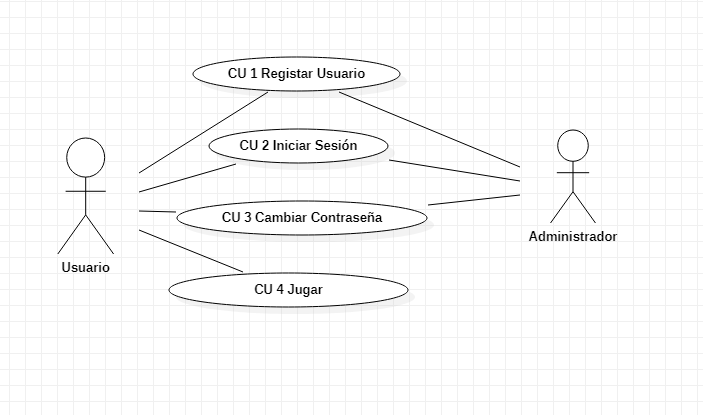
\includegraphics[scale=0.7]{imgs/CasosDeUso}
    \caption{Diagrama de Casos de Uso}
\end{figure}
\subsubsection{Tabla descriptiva de Caso de Uso 1}
\begin{table}[H]
\caption{Caso de Uso 1.}
\begin{tabular}{|M{4cm}|M{12cm}|}

\hline
Caso de Uso & CU1 Registrar Usuario\\ \hline
Versión & 1.1\\ \hline
Autor(es) & Itzcoatl Rodrigo Pineda Vieyra\\ \hline
Revisor & Izaird Alexander Mothelet Delgado \\ \hline
Actor(es) & Usuario Final \\ \hline
Entradas & correo electrónico, contraseña, \\ & Cuenta de Google \\ \hline
Salidas & Cuenta de usuario creada \\ \hline
Pre-condiciones & Instalar y abrir la aplicación \\ \hline
Post-condiciones & Cuenta de usuario creada\\ \hline
Mensajes & MSN1: "Ingrese un texto válido"\\
		 & MSN2: "Bienvenido"\\ \hline
Fuente & RF1,RF3 \\ \hline	
Trayectoria & 

Trayectoria A (principal)

\begin{enumerate}
\item El usuario seleccionará la opción de registrarse.
\item Se ingresarán los datos correspondientes.
\item Se creará correctamente la cuenta del usuario
\item Se envia un correo de confirmación al email proporcionado
\end{enumerate}

Trayectoria B

\begin{enumerate}
\item El usuario seleccionará la opción de registrarse.
\item Se proporcionará una cuenta de Google
\item Se confirma y se dan los permisos correspondientes.
\item Se creará correctamente la cuenta del usuario.
\end{enumerate}
\\ \hline
\end{tabular}
\end{table}

\subsubsection{Tabla descriptiva de Caso de Uso 2}
\begin{table}[H]
\caption{Caso de Uso 2.}
\begin{tabular}{|M{4cm}|M{12cm}|}
\hline
Caso de Uso & CU2 Iniciar Sesión\\ \hline
Versión & 1.1\\ \hline
Autor(es) & Itzcoatl Rodrigo Pineda Vieyra\\ \hline
Revisor & Izaird Alexander Mothelet Delgado \\ \hline
Actor(es) & Usuario Final \\ & Administrador\\ \hline
Entradas &  Correo electrónico, contraseña\\ & Cuenta de Google \\ \hline
Salidas & Sesión de usuario \\ \hline
Pre-condiciones & Instalar y abrir la aplicación \\ \hline
Post-condiciones & Sesión iniciada\\ \hline
Mensajes & MSN1: "Ingrese un texto válido"\\
		   & MSN2: "Bienvenido"\\ \hline
Fuente & RF2,RF3 \\ \hline	
Trayectoria & 

Trayectoria A (principal)

\begin{enumerate}
\item El usuario ingresa sus credenciales (correo y contraseña).
\item Se valida si existen coincidencias de las credenciales proporcionadas
\item Se inicia sesión o se despliega un mensaje de error.
\end{enumerate}

Trayectoria B

\begin{enumerate}
\item El usuario seleccionará la opción de registrarse.
\item Se proporcionará una cuenta de Google
\item Se inicia sesión.
\end{enumerate}
\\ \hline
\end{tabular}
\end{table}

\subsubsection{Tabla descriptiva de Caso de Uso 3}
\begin{table}[H]
\caption{Caso de Uso 3.}
\begin{tabular}{|M{4cm}|M{12cm}|}
\hline
Caso de Uso & CU3 Cambiar Contraseña\\ \hline
Versión & 1.1\\ \hline
Autor(es) & Itzcoatl Rodrigo Pineda Vieyra\\ \hline
Revisor & Izaird Alexander Mothelet Delgado \\ \hline
Actor(es) & Usuario Final \\ \hline
Entradas &  Correo y contraseña nueva \\ \hline
Salidas & Cuenta con contraeña nueva \\ \hline
Pre-condiciones & Iniciar Sesión \\ \hline
Post-condiciones & \\ \hline
Mensajes & MSN1: "Se envió el correo para restablecer contraseña"\\
		   & MSN2: "Bienvenido"\\ \hline
Fuente & RF4 \\ \hline	
Trayectoria &
\begin{enumerate}
\item El usuario selecciona Restablecer contraseña desde la pantalla principal.
\item Se envia el correo.
\item El usuario recibe un correo con una liga que le permita cambiar su contraseña.
\end{enumerate}
\\ \hline
\end{tabular}
\end{table}

\subsubsection{Tabla descriptiva de Caso de Uso 4}
\begin{table}[H]
\caption{Caso de Uso 4.}
\begin{tabular}{|M{4cm}|M{12cm}|}
\hline
Caso de Uso & CU4 Jugar\\ \hline
Versión & 1.1\\ \hline
Autor(es) & Itzcoatl Rodrigo Pineda Vieyra\\ \hline
Revisor & Izaird Alexander Mothelet Delgado \\ \hline
Actor(es) & Usuario Final \\ \hline
Entradas &  Respuesta, modo de juego, operación, dificultad \\ \hline
Salidas & Puntuación \\ \hline
Pre-condiciones & Iniciar Sesión \\ \hline
Post-condiciones & Puntuación\\ \hline
Mensajes & \\ \hline
Fuente & RF4, RF5 \\ \hline	
Trayectoria & 
\begin{enumerate}
\item El usuario selecciona Juegos del menú lateral o de la pantalla principal
\item El usuario selecciona el modo de juego, el tipo de operaciones y la dificultad.
\end{enumerate}

Trayectoria A Modo Clásico

\begin{enumerate}
\setcounter{enumi}{2}
\item El usuario responde  las preguntas 
\item Al completar una ronda de 10 preguntas o seleccionar el botón de finalizar termina el juego.
\item Se informa al usuario de su puntuación, mejor racha y tiempo y se registra la puntuación en el leaberboard
\end{enumerate}

Trayectoria B Modo Infinito

\begin{enumerate}
\setcounter{enumi}{2}
\item El usuario responde  las preguntas 
\item Al cometer 3 errores o seleccionar el botón de finalizar, termina el juego.
\item Se informa al usuario de su puntuación, mejor racha y tiempo y se registra la puntuación en el leaberboard
\end{enumerate} 

Trayectoria C Modo Jugador versus Jugador
\begin{enumerate}
\setcounter{enumi}{2}
\item Los usuarios responden las preguntas, el primero en responder correctamente recibe los puntos. 
\item Se informa a los usarios de su puntuación.
\end{enumerate} \\ \hline 
\end{tabular}
\end{table}

\subsubsection{Tabla descriptiva de Caso de Uso 5}
\begin{table}[H]
\caption{Caso de Uso 5.}
\begin{tabular}{|M{4cm}|M{12cm}|}
\hline
Caso de Uso & CU5 Consultar \emph{Leaderboard}\\ \hline
Versión & 1.1\\ \hline
Autor(es) & Itzcoatl Rodrigo Pineda Vieyra\\ \hline
Revisor & Izaird Alexander Mothelet Delgado \\ \hline
Actor(es) & Usuario Final \\ \hline
Entradas &  Modo de juego, operacion \\ \hline
Salidas & \emph{Leaderboard} \\ \hline
Pre-condiciones & Iniciar Sesión\\ \hline
Post-condiciones & \\ \hline
Mensajes & \\ \hline 
Fuente &  \\ \hline	
Trayectoria &
\begin{enumerate}
\item El usuario selecciona \emph{leaderboards} del menu lateral o de la pantalla principal 
\item El usuario selecciona el modo de juego, el tipo de operaciones.
\item Se despliega el \emph{leaderboard} correspondiente
\end{enumerate}
\\ \hline
\end{tabular}
\end{table}

\subsubsection{Tabla descriptiva de Caso de Uso 6}
\begin{table}[H]
\caption{Caso de Uso 6.}
\begin{tabular}{|M{4cm}|M{12cm}|}
\hline
Caso de Uso & CU6 Consultar Logros\\ \hline
Versión & 1.1\\ \hline
Autor(es) & Itzcoatl Rodrigo Pineda Vieyra\\ \hline
Revisor & Izaird Alexander Mothelet Delgado \\ \hline
Actor(es) & Usuario Final \\ \hline
Entradas &  Modo de juego, operación \\ \hline
Salidas & Logros \\ \hline
Pre-condiciones & Iniciar Sesión,  \\ \hline
Post-condiciones & \\ \hline
Mensajes & \\ \hline 
Fuente &  \\ \hline	
Trayectoria &
\begin{enumerate}
\item El usuario selecciona Logros del menú lateral o de la pantalla principal.
\item Se despliega la lista de logros 
\end{enumerate}
\\ \hline 
\end{tabular}
\end{table}

\subsubsection{Tabla descriptiva de Caso de Uso 7}
\begin{table}[H]
\caption{Caso de Uso 7.}
\begin{tabular}{|M{4cm}|M{12cm}|}

\hline
Caso de Uso & CU7 Subir Plantilla\\ \hline
Versión & 1.1\\ \hline
Autor(es) & Izaird Alexander Mothelet Delgado\\ \hline
Revisor &  Itzcoatl Rodrigo Pineda Vieyra \\ \hline
Actor(es) & Administrador \\ \hline
Entradas &  Plantilla, valores \\ \hline
Salidas & Plantilla \\ \hline
Pre-condiciones & Iniciar Sesión \\ \hline
Post-condiciones & Plantilla en Base de Datos\\ \hline
Mensajes & \\ \hline
Fuente &  \\ \hline	
Trayectoria &

\begin{enumerate}
\item El administrador selecciona Plantillas del menú lateral o de la pantalla principal.
\item Se despliega la lista de plantillas.
\item Se presiona el botón de + para agregar plantilla.
\item Se rellenan los campos de plantilla y valores respectivos a  cada dificultad.
\end{enumerate}
\\ \hline
		
\end{tabular}
\end{table}

\subsubsection{Tabla descriptiva de Caso de Uso 8}
\begin{table}[H]
\caption{Caso de Uso 8.}
\begin{tabular}{|M{4cm}|M{12cm}|}

\hline
Caso de Uso & CU7 Otorgar permisos\\ \hline
Versión & 1.1\\ \hline
Autor(es) & Itzcoatl Rodrigo Pineda Vieyra \\ \hline
Revisor &  Izaird Alexander Mothelet Delgado \\ \hline
Actor(es) & Administrador \\ \hline
Entradas &  Plantilla, valores \\ \hline
Salidas & 1 \\ \hline
Pre-condiciones & Iniciar Sesión  \\ \hline
Post-condiciones & Usuario con permisos de administrador\\ \hline
Mensajes & \\ \hline
Fuente &  \\ \hline	
Trayectoria &

\begin{enumerate}
\item El administrador selecciona Usuarios del menu lateral o de la pantalla principal.
\item Se despliega la lista de usuarios.
\item Se selecciona el usuario al que se desea otorgar o revocar permisos.
\item Se checa la checkbox para otorgar permisos.
\item Se selecciona la paloma para confirmar.
\end{enumerate}
\\ \hline
\end{tabular}

\end{table}


\subsection{Análisis de Interfaces}
%Descripcion de tipo de interfaz y por que
Las interfaces deberán ser optimizadas para dispositivos móviles. Deberá considerarse la capacidad \emph{touch} de dichos dispositivos. La primera pantalla será para Iniciar sesión por medio del correo y contraseña junto con un botón para registrarse. La pantalla de registro solicitará el correo, contraseña y confirmación de la contraseña. Se deberá contar con botones para acceder al perfil de usuario, \emph{leaderboards} y logros en una barra de navegación, esta puede ser horizontal o vertical. La pantalla de ejercicios mostrará la puntuación en todo momento en una esquina y el número de respuestas correctas consecutivas junto a un icono. En caso de haber tiempo para responder a una pregunta habrá una barra horizontal en la parte superior la cual irá desapareciendo conforme transcurra el tiempo asignado al usuario para dar respuesta a la pregunta.

\subsection{Análisis de la Base de Datos}%Narrativa
Para desarrollar esta aplicación se cuenta con una entidad Usuario con campos correo (llave primaria) y contraseña, con el correo como identificador de la entidad, pues no se permiten correos duplicados. Los Logros y leaderboards son manejados por el servicio externo de Google Play Juegos por lo cual no se incluyen en nuestra base de datos.

\subsection{Análisis de Logros}
Los logros son una manera de incentivar al jugador a cumplir ciertas metas, se decidió enfocarnos en pocos logros pero con un nivel de dificultad medio a difícil por recomendación del siguiente estudio \cite{groening2019achievement}.
Los logros se desbloquearán automáticamente al llegar a cierta puntuación, racha, o  responder rápido. Dando tres categorías de logros: Rachas, Tiempo, Puntuación. La puntuación es calculada en base a la dificultad y tiempo de respuesta de la siguiente forma: \(score = (a/b ) * c\) donde a es el tiempo de respuesta, b es el tiempo dado para 
der y c es la puntuación máxima por respuesta correcta.   Al completar todos los logros el progreso no se reestablecerá. 


\subsection{Tecnologías usadas}
\subsubsection{Dart}
Dart es un lenguaje optimizado para el cliente que permite desarrollar 
aplicaciones de una manera rápida y sencilla. Uno de sus objetivos principales es 
ofrecer un lenguaje de programación productivo para el desarrollo multiplataforma, 
junto con una plataforma de ejecución flexible.

Dart refuerza la programación orientada a objetos, como lenguaje de programación 
orientado a objetos, Dart designa cada valor del componente de la aplicación como 
un objeto. Hace hincapié en la herencia única de las clases, y cuenta con una sintaxis 
similar a la de otros lenguajes orientados a objetos como Swift y Objective-C.

En general, las interfaces orientadas a objetos se utilizan para convertir uno o varios 
componentes de la aplicación en objetos reutilizables, lo que permite realizar proyectos 
de codificación más avanzados y aislar los servicios de la aplicación. Estos objetos y 
las interfaces que los generan son una parte crucial de la introducción de la abstracción 
en una arquitectura, y también permiten la herencia múltiple, donde un solo objeto puede 
heredar características y rasgos de más de un objeto padre.

\subsubsection{Flutter}
Flutter es un kit de herramientas de interfaz de usuario portátil para crear 
aplicaciones de tipo nativo en móviles, web y escritorio, a partir de una 
única base de código. Utiliza el lenguaje de programación Dart e incorpora 
Material Design y los widgets de Cupertino. Los desarrolladores de Flutter 
pueden crear una interfaz de usuario espectacular que se ve y se siente 
nativa. Se comporta de forma natural en cualquier plataforma, a pesar de 
que está utilizando una sola base de código.

Flutter es el único framework con un SDK para móviles que proporciona un 
estilo \emph{responsive} sin utilizar un puente Javascript, alcanzando así un 
nivel de rendimiento que rivaliza con su primo y competidor directo 
React Native. Se integra fácilmente con las diferentes plataformas como 
Android, IOS y Linux, MAC, Windows y aplicaciones de Google Fuchsia.


\subsubsection{Firestore}
Firebase es un Backend-as-a-Service (Baas). Proporciona a los desarrolladores 
una variedad de herramientas y servicios para ayudarles a desarrollar aplicaciones 
de calidad. Está construido sobre la infraestructura de Google.

Firebase está categorizado como un programa de base de datos NoSQL, que almacena 
datos en documentos tipo JSON.

Firebase auth tiene un sistema de autenticación de correo electrónico/contraseña 
incorporado. También soporta OAuth2 para Google, Facebook, Twitter y GitHub. 


%\subsubsection{Google Play Servicies}
\subsection{Cierrre del capítulo}
Se describieron los requerimientos y casos de uso pertinentes a la aplicación lo cual se verá reflejaado en el diseño de la misma.
\pagebreak
\section{Diseño}
El diseño del sistema se centra en proporcionar la funcionalidad del sistema a través de sus diversos componentes, lo cual se expresa mediante diferentes diagramas, como se muestra en esta sección.
\subsection{Arquitectura general del sistema}%Imagen arquitectura y descripcion%Imagen arquitectura y descripcion
La arquitectura se compone de 4 subsistemas (ver figura 2).  El primer subsistema es el de Registro e inicio de sesión y es el encargado de dar de alta y permitir el acceso a los usuarios ya registrados. El segundo subsistema corresponde a los módulos que interactúan con el usuario, estos son el módulo de ejercicios, encargado de proporcionar ejercicios al usuario, y el módulo evaluador de logros y mecánicas, el cual se encarga de llevar el registro de la puntuación, logros y niveles. El Subsistema de administrador incluye los módulos generador de problemas y evaluador de expresiones, los cuales se usan para generar los ejercicios para el usuario. También se incluye un módulo de actualización y consulta de dichos ejercicios. El último subsistema es el de estadísticas y progreso, el cual lleva el registro de los logros globales del usuario.  
\begin{figure}[H]
    \centering
    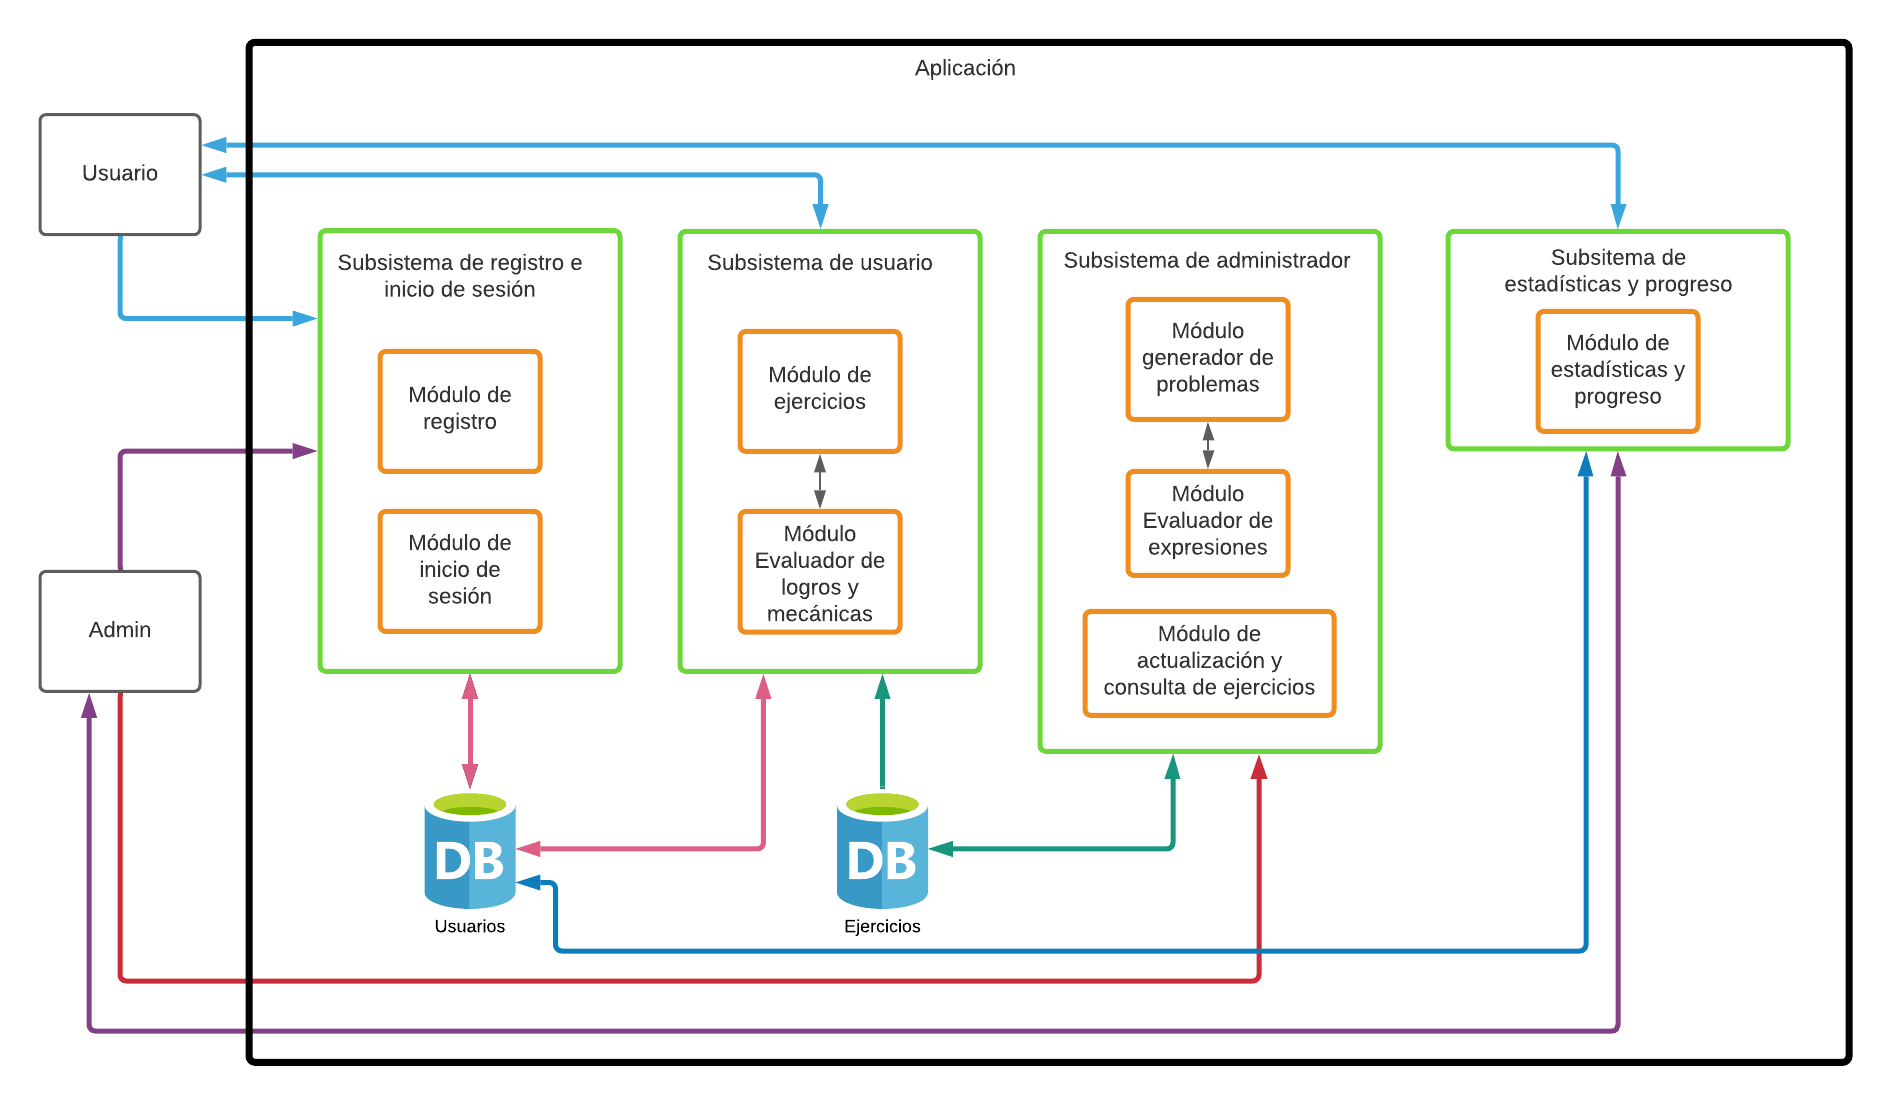
\includegraphics[scale=0.65]{imgs/Arquitectura}
    \caption{Arquitectura}
\end{figure}

\subsection{Diseño de Base de Datos}%diagrama entidad relacion pk subrayada
\begin{figure}[H]
    \centering
    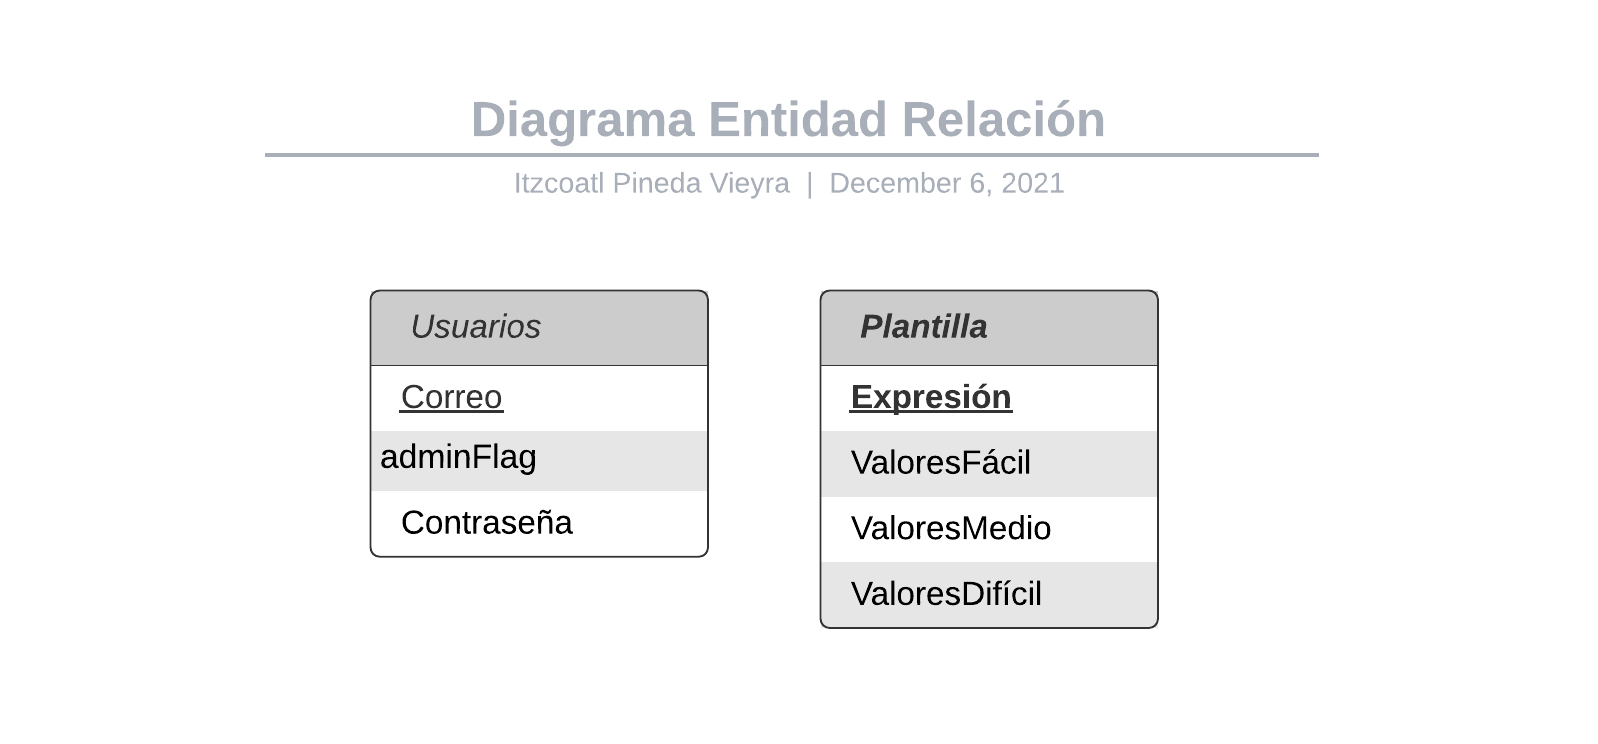
\includegraphics[scale=0.9]{imgs/BSD}
    \caption{Diagrama entidad relación}
\end{figure}
\subsection{Diseño de Logros}
Los logros que se incluyeron se muestran en la tabla 10.

\begin{table}[H]
\caption{Tabla de Logros}	
\begin{tabular}{|M{5cm}|p {12cm} |}
\hline
Logro & Descripción\\ \hline
Inspirado & Consigue una racha de al menos 5 en el modo Infinito\\ \hline
Ascendido & Consigue una racha de al menos 10 respuestas correctas en el modo Infinito\\ \hline
Perfeccionista & Responde correctamente todas las preguntas en una ronda del modo Clásico\\ \hline
Ágil &  En el modo Clásico, termina una partida en menos de 3 minutos con al menos 7 respuestas correctas.\\ \hline
Veloz & En el modo Clásico, termina una partida en menos de 2 minutos con al menos 7 respuestas correctas.\\ \hline
Sub60s &   En el modo Clásico, termina una partida en menos de 1 minuto con al menos 7 respuestas correctas.\\ \hline
Académico & Consigue una puntuación de al menos 2,500 en el modo Clásico, dificultad Fácil\\ \hline
Estudioso & Consigue una puntuación de al menos 5,000 en el modo Clásico, dificultad Medio\\ \hline
Erudito & Consigue una puntuación de al menos 10,000 en el modo Clásico, dificultad Difícil\\ \hline
	
\end{tabular}
\label{tab:Logros}

\end{table}
\subsection{Diseño de Interfaces}%mock-ups
En este apartado se presentan los diseños de las interfaces previamente descritas.
\pagebreak

En la figura 4 se muestra la pantalla de registro donde se piden los datos necesarios para crear una cuenta
\begin{figure}[H]
    \centering
    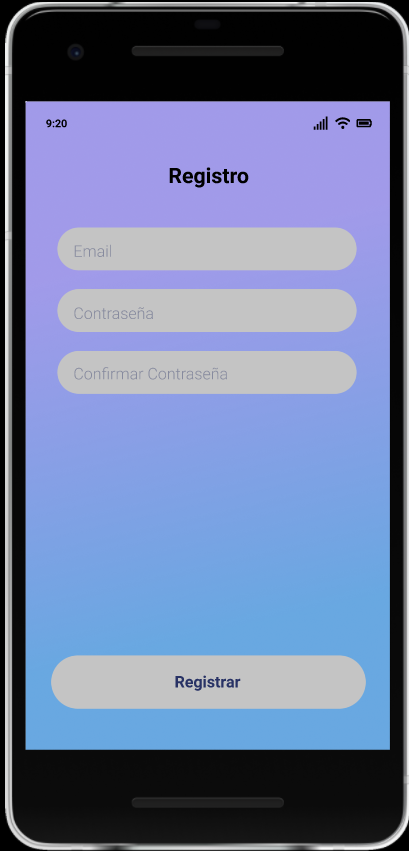
\includegraphics[scale=0.7]{imgs/Figma/Registro2} 
    \caption{Registro}
\end{figure}
\begin{figure}[H]
    \centering
    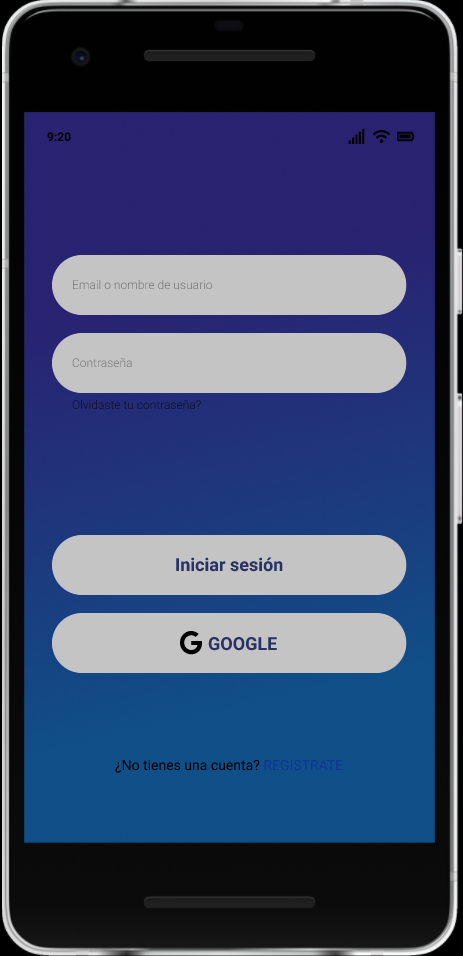
\includegraphics[scale=0.8]{imgs/Figma/Login}
    \caption{Login}
\end{figure}
En la figura 6 se presenta la pantalla en la que se otorgan permisos al administrador.
\begin{figure}[H]
    \centering
    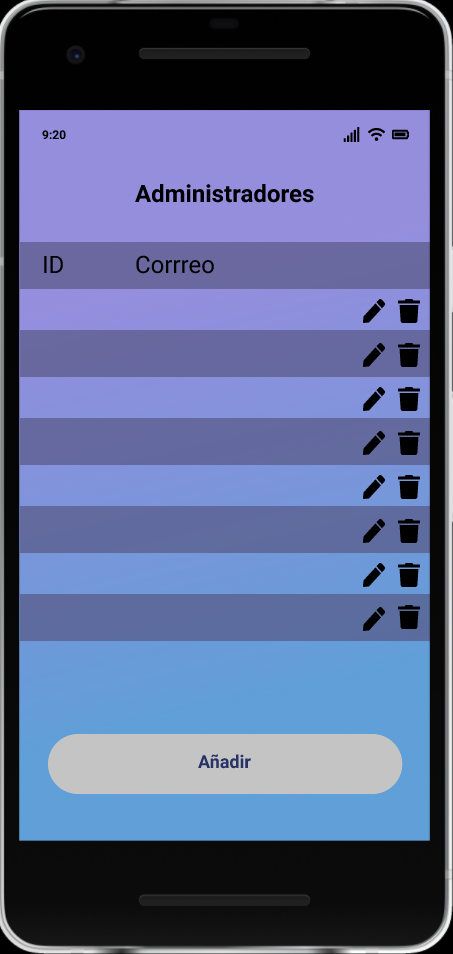
\includegraphics[scale=0.8]{imgs/Figma/Admins}
    \caption{Administrador}
\end{figure}
En la figura 7 se muestra que datos se requieren para crear una plantilla.
\begin{figure}[H]
    \centering
    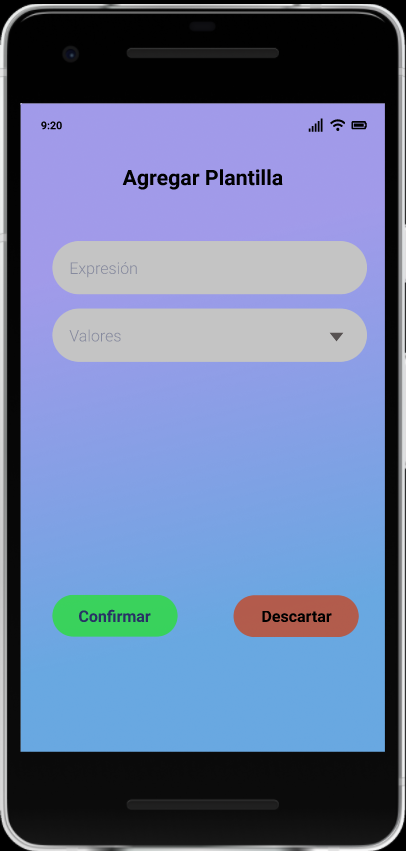
\includegraphics[scale=0.8]{imgs/Figma/Plantilla}
    \caption{Plantillas}
\end{figure}

\begin{figure}[H]
    \centering
    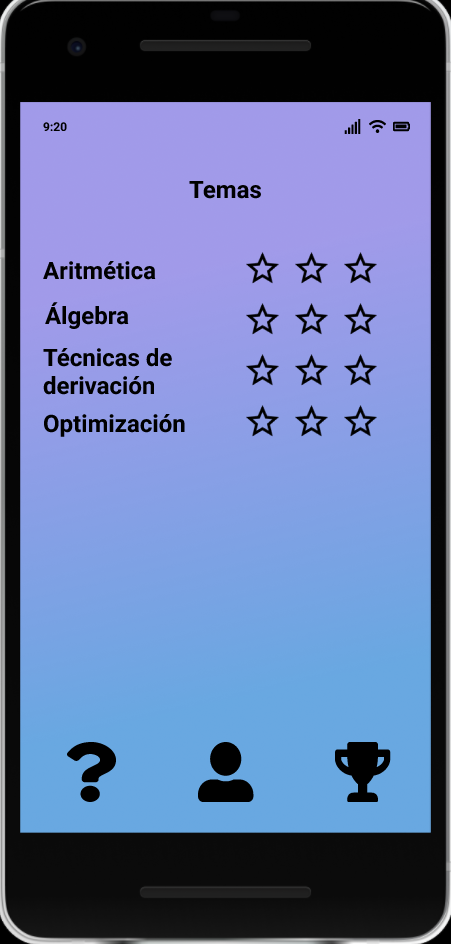
\includegraphics[scale=0.8]{imgs/Figma/Temas}
    \caption{Selección de tema}
\end{figure}
Esta pantalla es un ejemplo del modo de juego
\begin{figure}[H]
    \centering
    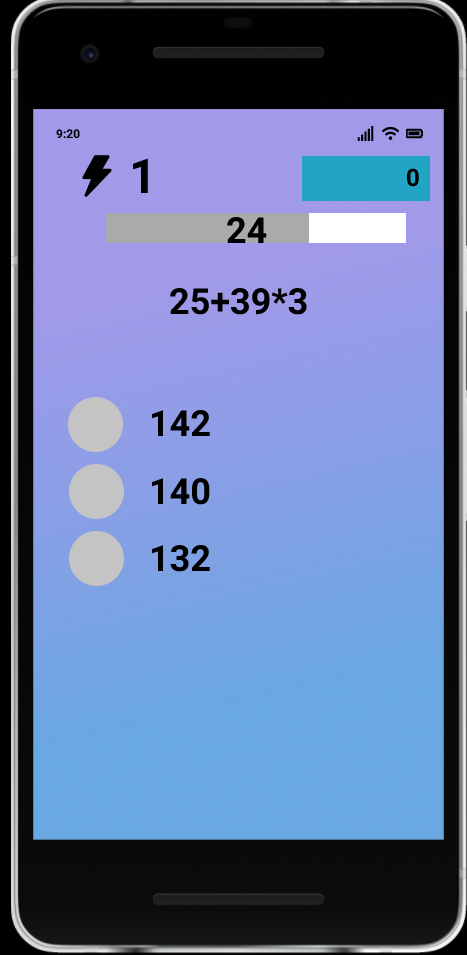
\includegraphics[scale=0.8]{imgs/Figma/Ejemplo}
    \caption{Ejemplo}
\end{figure}
\begin{figure}[H]
    \centering
    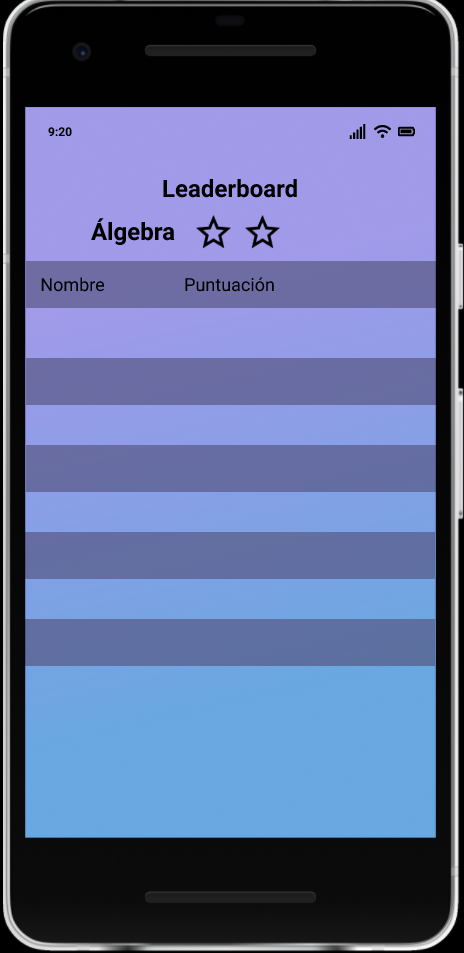
\includegraphics[scale=0.8]{imgs/Figma/Leaderboard}
    \caption{Leaderboard}
\end{figure}
\begin{figure}[H]
    \centering
    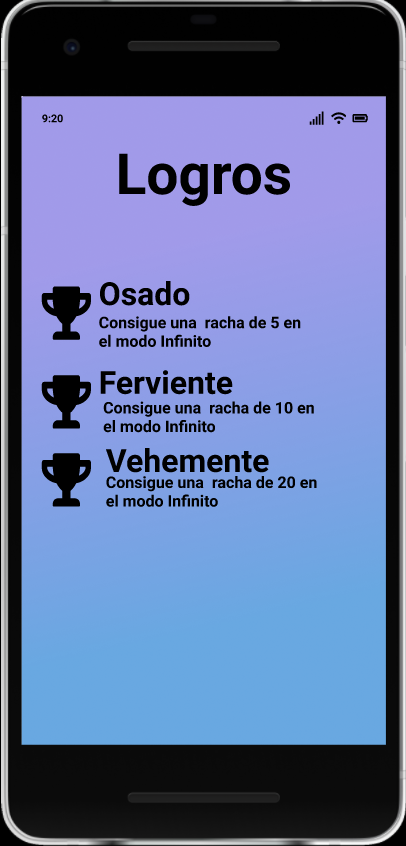
\includegraphics[scale=0.9]{imgs/Figma/Logros}
    \caption{Logros}
\end{figure}

\pagebreak
\section{Implementación}
%Subsistema de registro e ingreso Captura de pantalla con descripcion citar mock up de la pantalla
El subsistema de registro e ingreso fue implementado con Firebase 
\begin{figure}[H]
    \centering
    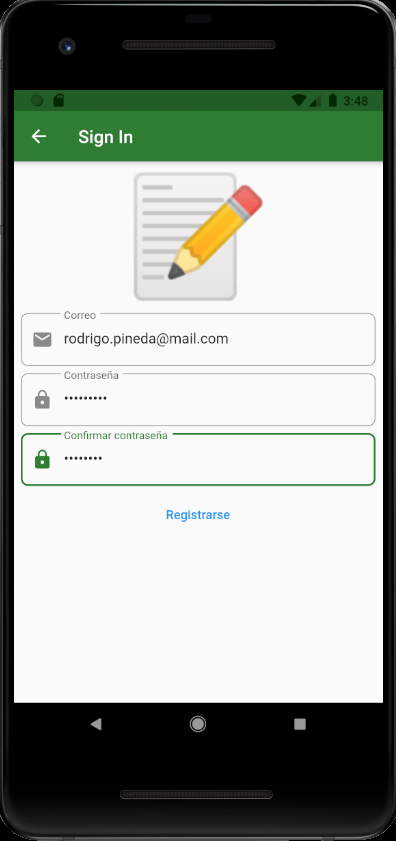
\includegraphics[scale=0.8]{imgs/Imp/Registro}
    \caption{Implementación Registro}
\end{figure}
\begin{figure}[H]
    \centering
    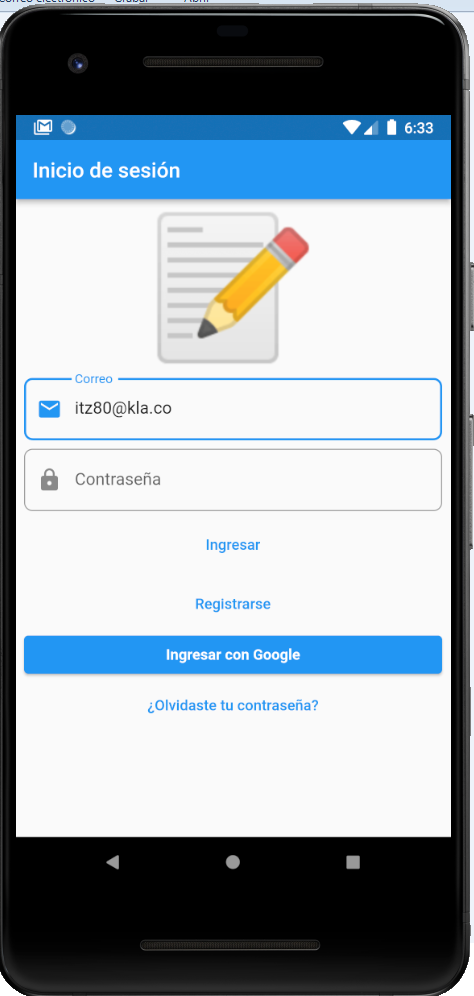
\includegraphics[scale=0.8]{imgs/Imp/Login1}
    \caption{Implementación de Login}
\end{figure}
Pantalla principal de usuario.
\begin{figure}[H]
    \centering
    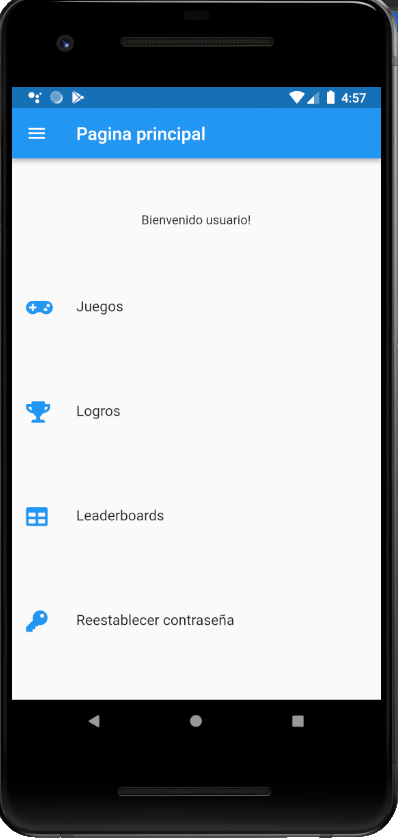
\includegraphics[scale=0.8]{imgs/Imp/MainUsuario}
    \caption{Pantalla Principal de Usuario}
\end{figure}
Ejemplo de modo de juego Jugador versus Jugador, el modo esta diseñado para que dos usuarios jueguen en el mismo dispositivo.
\begin{figure}[H]
    \centering
    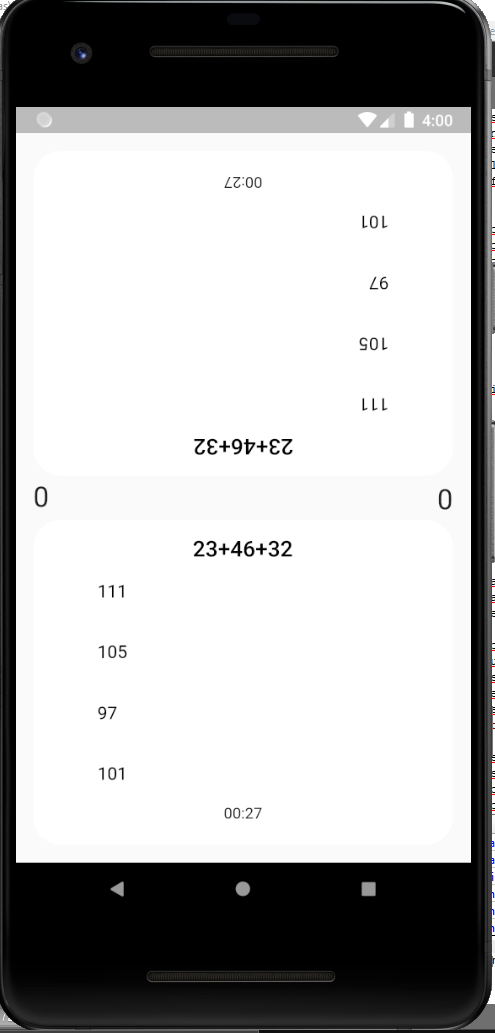
\includegraphics[scale=0.8]{imgs/Imp/Pvp}
    \caption{Implementación de modo jugador contra jugador}
\end{figure}
Ejemplo de modo infinito.
\begin{figure}[H]
    \centering
    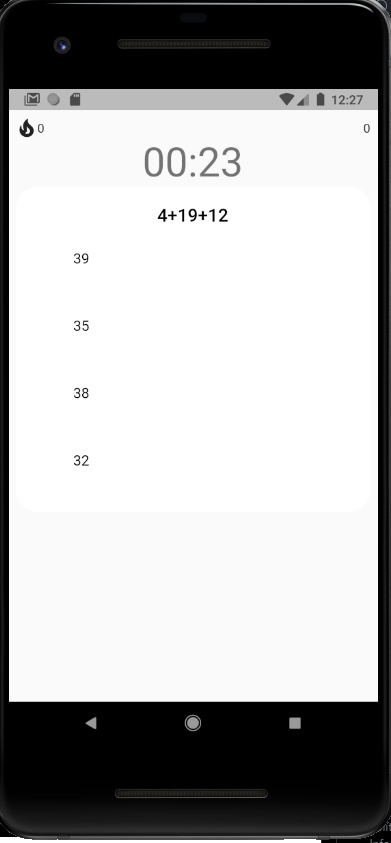
\includegraphics[scale=0.8]{imgs/Imp/Endless}
    \caption{Implementación de modo infinito}
\end{figure}
\begin{figure}[H]
    \centering
    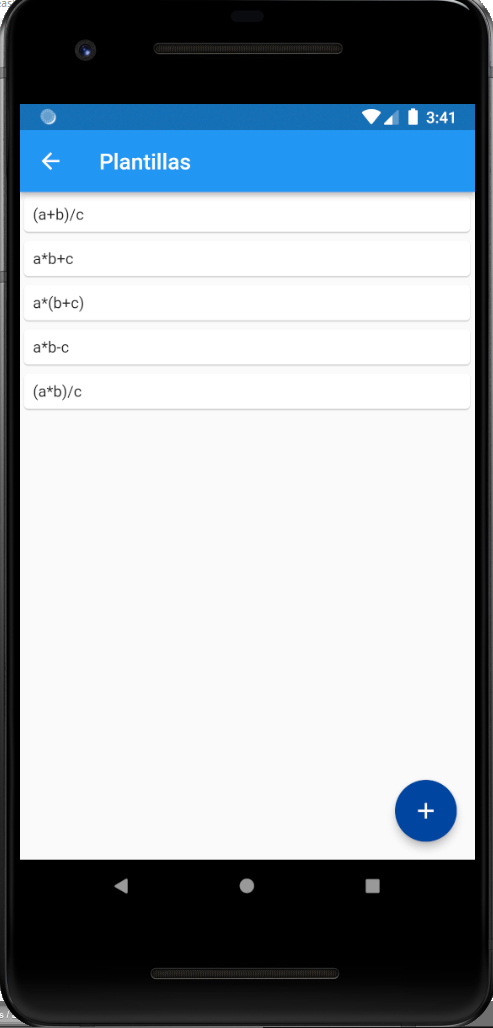
\includegraphics[scale=0.8]{imgs/Imp/Plantillas}
    \caption{Implementación de Plantillas}
\end{figure}
\begin{figure}[H]
    \centering
    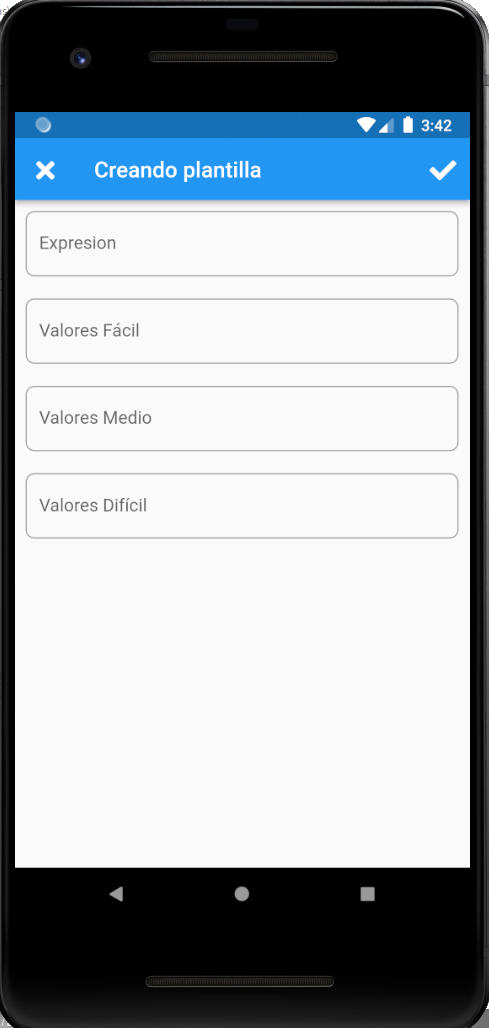
\includegraphics[scale=0.8]{imgs/Imp/Plantillas2}
    \caption{Implementación de Plantillas}
\end{figure}
\begin{figure}[H]
    \centering
    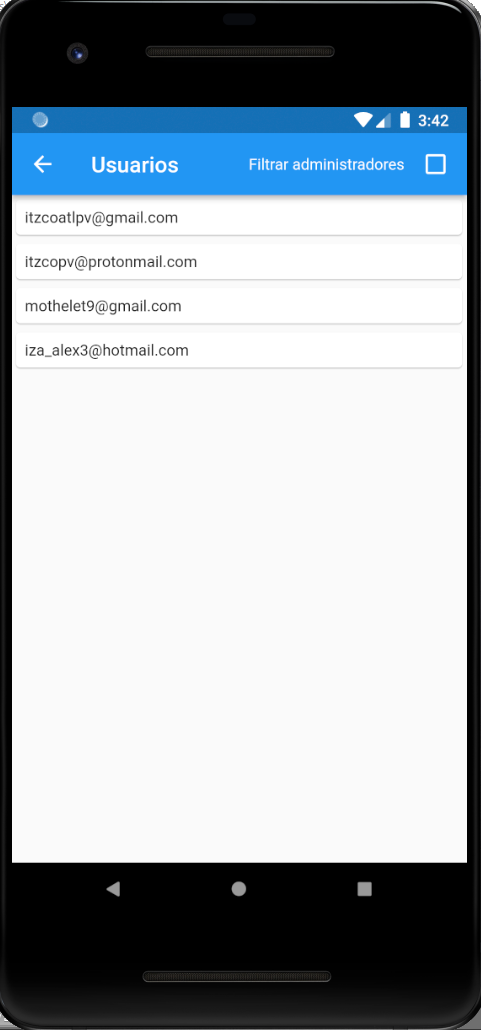
\includegraphics[scale=0.8]{imgs/Imp/Usuarios}
    \caption{Implementación de Usuarios}
\end{figure}
\begin{figure}[H]
    \centering
    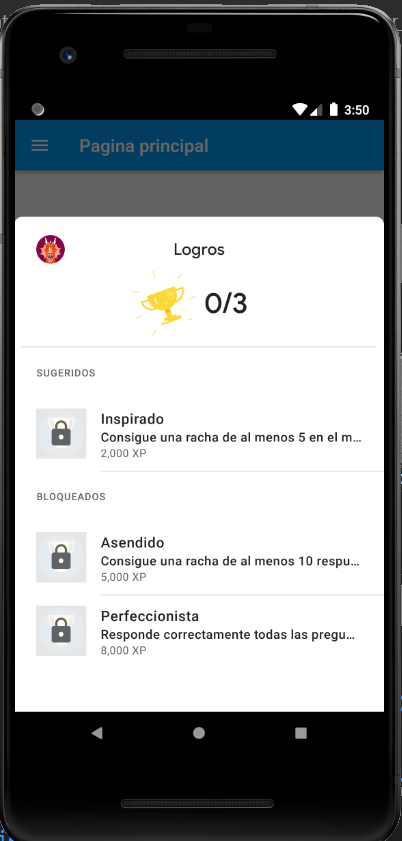
\includegraphics[scale=0.8]{imgs/Imp/Logros}
    \caption{Implementación de Logros}
\end{figure}
\begin{figure}[H]
    \centering
    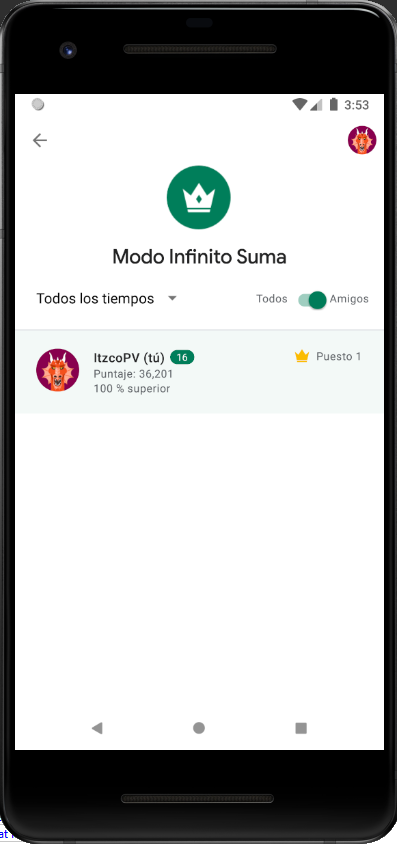
\includegraphics[scale=0.8]{imgs/Imp/Leaderboards}
    \caption{Implementación de Leadorboards}
\end{figure}


\section{Pruebas}
En esta sección se reportan los resultados obtenidos de las pruebas realizadas a la 
aplicación.

Las primeras pruebas fueron las correspondientes a la funcionalidad del sistema y 
un segundo tipo de pruebas fueron efectuadas, con el objetivo de tener una mejor 
visión acerca de la experiencia de usuario y la usabilidad de la aplicación.

\subsection{Pruebas de funcionalidad}
Se validó el correo con una expresión regular. Algunos ejemplos de correos validos
\begin{itemize}
	\item itz80@kla.co
	\item \verb |itz!&*%^7@protonmail.net|
	\item 1A!e@protonmail.com
\end{itemize}
Se valido la capacidad de desbloquear logros como se puede observar en las figuras
\ref{fig:pruebas_01}, \ref{fig:pruebas_02} y \ref{fig:pruebas_03}
\begin{figure}[H]
    \centering
    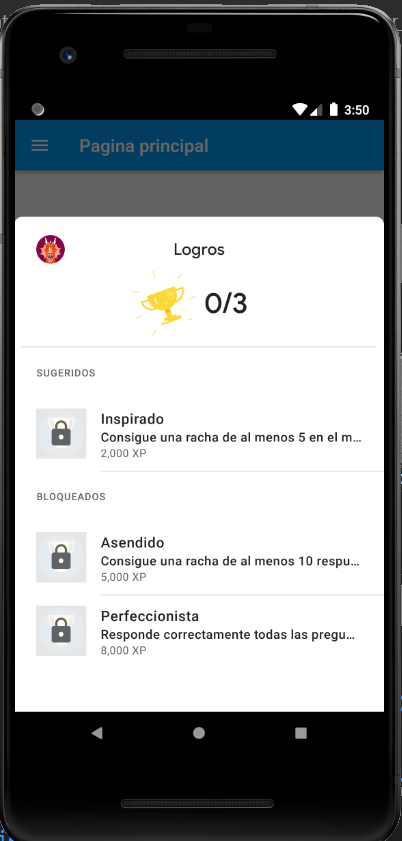
\includegraphics[scale=0.8]{imgs/Imp/Logros}
    \caption{Logros sin desbloquear}
    \label{fig:pruebas_01}
\end{figure}
\begin{figure}[H]
    \centering
    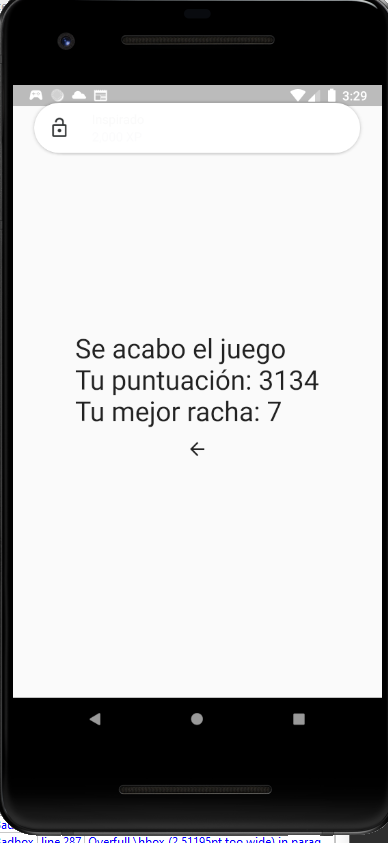
\includegraphics[scale=0.8]{imgs/Test/LogroDes}
    \caption{Cumpliendo la condición}
    \label{fig:pruebas_02}
\end{figure}
\begin{figure}[H]
    \centering
    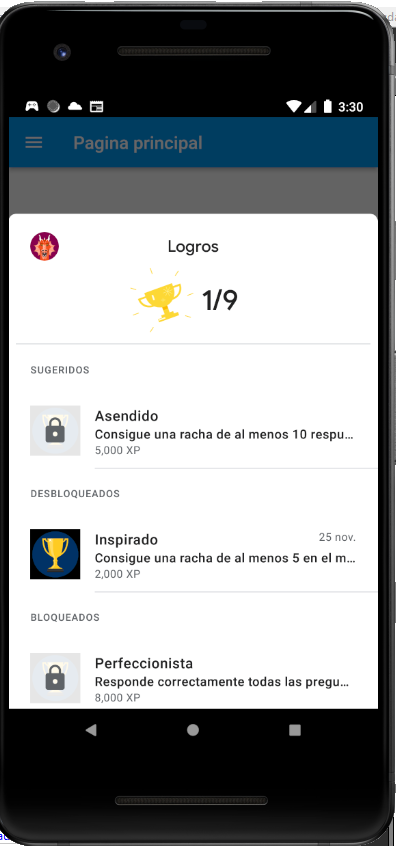
\includegraphics[scale=0.8]{imgs/Test/LogroDes2}
    \caption{Logros Desbloqueado}
    \label{fig:pruebas_03}
\end{figure}

\subsection{Pruebas de experiencia de usuario y de usabilidad}
La experiencia de usuario (expresada como UX por su nombre en inglés user experience), 
describe los sentimientos subjetivos de los usuarios hacia los productos que utilizan. 
Diferentes usuarios pueden tener diferentes impresiones con respecto a la UX del mismo 
producto. Por lo que es necesario medir la UX de un grupo para tener mayor confianza 
en los resultados\cite{santoso2016measuring}.

Para realizar dichas mediciones, Lewis menciona \cite{lewis2018item} que el 
cuestionario de la Escala de Usabilidad de Sistemas o SUS por sus siglas en 
inglés (System Usability Scale), se ha vuelto una valiosa herramienta, ya que permite 
evaluar la usabilidad y la experiencia del usuario. Por su parte, Sauro 
mostró\cite{ng2011measuring} que SUS es un cuestionario de usabilidad válido y 
confiable. 

El SUS es un cuestionario estandarizado de diez preguntas con cinco opciones 
para responder, el rango de medición de las respuestas va de totalmente en desacuerdo 
a totalmente de acuerdo y los valores van de 1 a 5 respetivamente. Los valores 
obtenidos se homogenizan  usando las siguientes fórmulas: 

\begin{center}
$ V_{i}-1 \textrm{ , si el reactivo es impar (1)} $

$ 5-V_{i} \textrm{ , si el reactivo es par (2)} $
\end{center}

Donde: $V_{i}$ representa el valor obtenido inicialmente, indexado por i.

La evaluación del cuestionario permite clasificar la usabilidad de la herramienta 
tecnológica educativa, empleando las siguientes operaciones: Los valores transformados 
de las respuestas obtenidas, primeramente se suman, para después multiplicarse por 
el factor 2.5. Los resultados obtenidos que sean mayores a 68, pero menores de 80.3, 
se consideran superiores al promedio o se califican con el adjetivo “Bueno”, lo que 
implica que la herramienta evaluada cumple con los atributos de calidad requeridos. 
Si se obtiene una puntuación mayor a 80.3 es considerada como “Excelente” 
\cite{derisma2020usability}. 
Obsérvese la tabla \ref{tab:pruebas01}.

\begin{table}[H]
\centering
\begin{tabular}{|c|c|}
\hline
Evaluación SUS Rango & Evaluación SUS en Adjetivo \\ \hline
$>$80.3 & Excelente \\ \hline
68 – 80.3 & Bueno \\ \hline
68	& Suficiente \\ \hline 
51 – 68 & Pobre \\ \hline 
$<$51 & Muy deficiente \\ \hline
\end{tabular}
\caption{Rango de evaluación del cuestionario SUS}
\label{tab:pruebas01}
\end{table}


Los valores obtenidos inicialmente de las preguntas pares se encuentran en “código inverso” 
con respeto a los valor	es obtenidos inicialmente por las preguntas pares, es por esto por 
lo que se requieren homogenizar. 

El cuestionario SUS mide los atributos de la usabilidad, y de acuerdo con Nielsen \cite{nielsen1994usability}
la usabilidad es definida por 5 componentes de calidad: 

\begin{enumerate}
\item Aprendizaje. Se refiere a la facilidad que tienen los usuarios para realizar las 
tareas básicas desde la primera vez que trabajan con el sistema. 
\item Eficiencia. Consiste en lo que los usuarios han aprendido para usar el sistema, 
así como a la rapidez con la que realizan las tareas. 
\item Memorabilidad. Facilidad con la que el usuario recuerda el funcionamiento del 
sistema después de un periodo de tiempo de no usarlo.
\item Tasa de errores. Es la cantidad de errores cometidos por los usuarios durante 
el empleo del sistema, enfocándose en la gravedad de los mismos, así como en la 
facilidad con la que pueden recuperarse después de haber cometido un error.
\item Satisfacción. Implica lo agradable que representa para el usuario el uso del 
sistema.
\end{enumerate}

Para la realización de este estudio se trabajó con un grupo de 18 estudiantes de nivel 
superior de segundo semestre, quienes trabajaron con la aplicación durante dos días, 
en sus tiempos libres, y al tercer día resolvieron el cuestionario SUS. Es importante 
señalar que todas las indicaciones se dieron a distancia empleando la plataforma de 
zoom (figuras 1, 2 y 3). Se agregó una pregunta al cuestionario SUS, lo que brindó 
información extra sobre la aplicación. Los participantes resolvieron el cuestionario 
vía online a través de Google Forms. Para el análisis de los datos se empleó Excel. 


\begin{figure}[H]
    \centering
    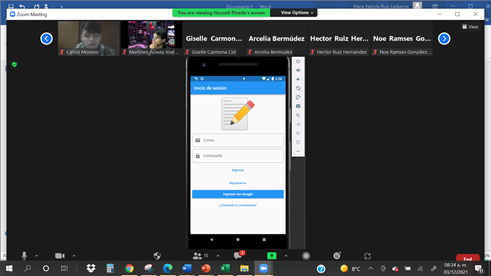
\includegraphics[scale=0.7]{imgs/pruebas/pruebas_01.png}
    \caption{Explicación de la navegación por la aplicación}
\end{figure}

\begin{figure}[H]
    \centering
    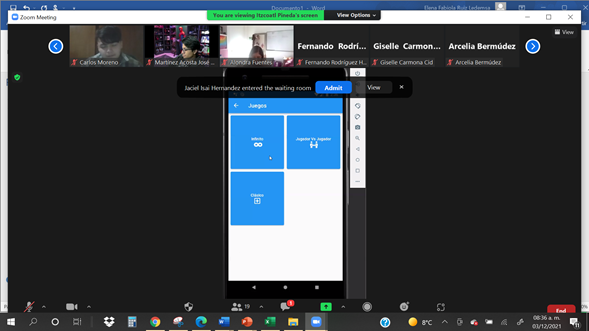
\includegraphics[scale=0.7]{imgs/pruebas/pruebas_02.png}
    \caption{Explicación de la realización de operaciones en la aplicación}
\end{figure}

\begin{figure}[H]
    \centering
    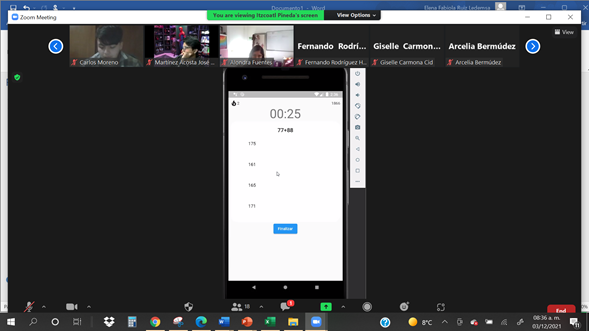
\includegraphics[scale=0.7]{imgs/pruebas/pruebas_03.png}
    \caption{Explicación de las instrucciones para trabajar con la aplicación}
\end{figure}

Después de haber aplicado el cuestionario se descargó el archivo generado por la plataforma 
Google Forms con extensión .csv y se convirtió en uno .xls para comenzar con el tratamiento 
de los datos. Para la evaluación del cuestionario SUS, primeramente, se usaron las fórmulas 
1 y 2 para homogenizar los datos de los valores obtenidos inicialmente por los reactivos de 
cada pregunta, a continuación, se sumaron los resultados de cada participante, para luego 
multiplicarse por 2.5. Se continúo el cálculo, sumando los puntajes de los participantes y 
promediándolos. 

Por último, se comparó el resultado final con la clasificación de los rangos de evaluación 
en la escala de usabilidad del cuestionario SUS, obteniéndose una puntuación de 79.58 de 
aceptación, en relación a la usabilidad que los participantes tuvieron al trabajar con la 
aplicación, por lo que está en el rango de “Bueno”. En el tabla \ref{tab:pruebas02} se aprecian los valores 
obtenidos.

\begin{table}[H]
\centering
\begin{tabular}{|c|c|c|c|c|c|c|c|c|c|c|c|}
\hline
P1 & P2 & P3 & P4 & P5 & P6 & P7 & P8 & P9 & P10 & SUMA & PRODCUTO CON 2.5\\ \hline
2 & 1 & 2 & 2 & 2 & 4 & 4 & 4 & 2 & 3 & 26 & 65\\ \hline
2 & 1 & 3 & 4 & 3 & 4 & 3 & 4 & 2 & 4 & 30 & 75\\ \hline
2 & 1 & 4 & 4 & 2 & 4 & 4 & 4 & 1 & 4 & 30 & 75\\ \hline
2 & 1 & 4 & 4 & 3 & 4 & 4 & 4 & 0 & 4 & 30 & 75\\ \hline
2 & 2 & 4 & 4 & 4 & 4 & 4 & 4 & 3 & 4 & 35 & 87.5\\ \hline
2 & 2 & 4 & 4 & 3 & 2 & 4 & 4 & 2 & 4 & 31 & 77.5\\ \hline
3 & 4 & 4 & 4 & 3 & 4 & 4 & 4 & 4 & 4 & 38 & 95\\ \hline
3 & 0 & 4 & 3 & 3 & 3 & 4 & 4 & 4 & 4 & 32 & 80\\ \hline
2 & 4 & 4 & 3 & 3 & 4 & 3 & 4 & 4 & 3 & 34 & 85\\ \hline
3 & 3 & 4 & 3 & 3 & 4 & 4 & 4 & 4 & 3 & 35 & 87.5\\ \hline
3 & 4 & 3 & 4 & 3 & 4 & 3 & 4 & 3 & 4 & 35 & 87.5\\ \hline
3 & 3 & 4 & 3 & 3 & 3 & 4 & 4 & 4 & 3 & 34 & 85\\ \hline
3 & 1 & 3 & 1 & 3 & 4 & 3 & 1 & 3 & 1 & 23 & 57.5\\ \hline
2 & 3 & 2 & 3 & 2 & 3 & 3 & 4 & 1 & 3 & 26 & 65\\ \hline
2 & 4 & 3 & 3 & 3 & 2 & 3 & 3 & 3 & 2 & 28 & 70\\ \hline
2 & 2 & 3 & 3 & 4 & 4 & 4 & 4 & 4 & 3 & 33 & 82.5\\ \hline
4 & 4 & 4 & 4 & 4 & 4 & 4 & 4 & 4 & 4 & 40 & 100\\ \hline
1 & 2 & 3 & 4 & 2 & 3 & 4 & 4 & 4 & 4 & 33 & 82.5\\ \hline
2 & 1 & 2 & 2 & 2 & 4 & 4 & 4 & 2 & 3 & 26 & 65\\ \hline
  &   &   &   &   &   &   &   &   &   &    & 79.58\\ \hline
\end{tabular}
\caption{Valores de las respuestas a los reactivos del cuestionario SUS}
\label{tab:pruebas02}
\end{table}


Con el anterior resultado se evaluaron 4 de los 5 componentes de calidad que integran 
a la usabilidad, que son: fácil de aprender, fácil de recordar, baja taza de errores 
y satisfacción. Esta información aparece en la Tabla \ref{tab:pruebas03}.

\begin{table}[H]
\centering
\begin{tabular}{|l|M{10cm}|l|}
\hline
\multicolumn{3}{|c|}{Cuestionario de Escala de Usabilidad de Sistemas (SUS)} \\ \hline
Clave & Preguntas & Atributo \\ \hline
R1 & Creo que usaré esta plataforma o sistema frecuentemente. & Satisfacción\\ \hline
R2 & Encuentro la plataforma o sistema innecesariamente complejo. & Memoria\\ \hline
R3 & Pienso que la plataforma o sistema fue fácil de usar.  & Memoria\\ \hline
R4 & Pienso que voy a necesitar soporte técnico para poder usar esta plataforma o sistema. & Error\\ \hline
R5 & Encontré varias funciones en la plataforma o sistema bien integradas.  & Aprendizaje\\ \hline
R6 & Pienso que hubo muchas inconsistencias en el sistema o plataforma. & Error \\ \hline
R7 & Imagino que la mayoría de las personas podrían aprender a usar esta plataforma o sistema bastante rápido.   & Aprendizaje\\ \hline
R8 & Encuentro la plataforma o sistema muy molesto de usar. & Satisfacción\\ \hline
R9 & Me siento muy seguro al usar la plataforma o sistema.  & Satisfacción\\ \hline
R10 & Siento que necesitaré que aprender muchas cosas antes de que pueda utilizar correctamente la plataforma o sistema. & Aprendizaje\\ \hline
\end{tabular}
\caption{Cuestionario de Escala de Usabilidad de Sistemas (SUS)}
\label{tab:pruebas03}
\end{table}


Los ítems que representan al atributo de Satisfacción son R1, R8 y R9. En la tabla \ref{tab:pruebas03} 
se observa que los estudiantes consideran emplear frecuentemente la aplicación, debido, 
entre otros factores, a que es segura y se sienten a gusto con ella. La puntuación 
obtenida es de 3.3 para el uso frecuente de la plataforma, en una escala de 1 a 5, 
en donde 1 es muy en desacuerdo y 5 es muy de acuerdo. La seguridad que les causa 
el empleo de la aplicación tiene un valor de 3.7 y la del gusto que les causa su 
uso también es de 3.7, en la misma escala de 1 a 5. Los puntajes obtenidos del 
promedio, sobre pasan el valor de 3 y la variabilidad de los datos con respecto a 
la media no pasa de 1, por lo que se considera que el nivel de satisfacción de la 
aplicación es bueno.

Con respecto al atributo de Aprendizaje, los reactivos que lo evaluaron son R5, R7 y R10. 
Los estudiantes de la muestra consideran que la curva de aprendizaje del uso de la 
aplicación, es baja debido a que las funciones están bien integradas, así como a la 
rapidez con la que aprendieron a usar los distintos componentes de la aplicación. 
Los valores de los promedios referidos a una buena integración de las funciones y 
de la rapidez de su uso puntuó en 3.9 cada una en una escala de 1 a 5. Concluyéndose 
que la forma de trabajar con la aplicación es prácticamente intuitiva.

En cuanto al atributo de Memoria, este fue evaluado a través de los reactivos R2 y R3, 
los estudiantes de la muestra estuvieron de acuerdo en que la aplicación fue fácil de 
usar con una puntuación de 4.4 y estuvieron en desacuerdo en que la plataforma fuera 
innecesariamente compleja con una puntuación de 1.78 en la misma escala empleada de 
1 a 5, por lo que ambos resultados se consideran buenos para la aplicación.

Finalmente, los reactivos restantes que son R4 y R6, los cuales evalúan la cantidad 
de errores que se pueden generar al interactuar con la aplicación. Los valores 
obtenidos en el cuestionario fueron 1.67 y 1.16 en una escala de 1 a 5, por lo que 
se interpreta que los estudiantes estuvieron muy en desacuerdo en necesitar soporte 
técnico como el que existieran inconsistencias en la aplicación.



\begin{table}[H]
\centering
\begin{tabular}{|l|l|l|l|}
\hline
Clave & Promedio por Pregunta & & Rango en la evaluación \\ \hline
R1 & 3.33 & 0.77 & De acuerdo \\ \hline
R2 & 1.78 & 1.22 & En desacuerdo\\ \hline
R3 & 4.44 & 0.70 & De acuerdo \\ \hline
R4 & 1.67 & 0.84 & Muy de acuerdo \\ \hline
R5 & 3.94 & 0.64 & De acuerdo \\ \hline
R6 & 1.16 & 0.92 & Totalmente en descuerdo \\ \hline
R7 & 4.67 & 0.49 & Totalmente de acuerdo \\ \hline
R8 & 1.22 & 0.73 & Muy en desacuerdo \\ \hline
R9 & 3.689 & 1.28 & De acuerdo \\ \hline
R10 & 1.61 & 0.85 & En desacuerdo \\ \hline
\end{tabular}
\caption{Valores estadísticos del cuestionario SUS}
\label{tab:pruebas04}
\end{table}


\pagebreak\section{Referencias}

\printbibliography[heading=none]

\end{document}
